\begingroup
\setlength{\emergencystretch}{2em}
\capituloTesis{Resultados}


Los resultados se organizaron según las cuatro relaciones planteadas entre la condición del drenaje vial y el desempeño funcional del pavimento en el tramo EMP.LI105 Pedregal–Censo–Cumbray, Simbal, 2026; en este orden de ideas, primero se presenta la identificación de las unidades estructura–sector y la verificación de sus indicadores, para continuar con la distribución de continuidad longitudinal (CL), abertura transversal libre (CT), índice de condición del pavimento (PCI) e índice internacional de rugosidad (IRI), y finalmente con las correlaciones y los contrastes bajo un modelo nulo espacial. De esta manera, la secuencia permite distinguir los resultados numéricos de las decisiones inferenciales y conserva la correspondencia entre cada hipótesis y los datos utilizados para examinarla.

Considerando la correspondencia requerida entre drenaje y pavimento, la base analítica se consolidó en veinte unidades estructura–sector identificadas del SIM-01 al SIM-20, distribuidas en cuatro tramos; sus mediciones originales comprendieron los márgenes del drenaje longitudinal, los extremos de cada estructura transversal, las subunidades de inspección superficial y los recorridos de perfilado. De esta manera, los registros subordinados se integraron en una fila por unidad para evitar tratarlos como observaciones independientes, mientras que los cuatro contrastes específicos se evaluaron con un nivel de significancia familiar de 0,05 y corrección de Holm sobre los valores obtenidos mediante aleatorización espectral de Moran.

\seccionTesis{Caracterización del corredor y delimitación de la base de análisis}

El orden de presentación responde a la secuencia de los cuatro objetivos específicos: inicialmente se caracteriza la composición del conjunto y se examina la integridad de las mediciones, luego se describen las distribuciones de las dos dimensiones de drenaje y de los dos indicadores funcionales, y finalmente se analizan las correspondencias CL–PCI, CL–IRI, CT–PCI y CT–IRI. La distinción entre coeficientes convencionales y coeficientes de rangos ajustados por coordenadas se mantiene en todo el capítulo para que sus valores no se interpreten como estimaciones intercambiables.

\subseccionTesis{Distribución de las unidades estructura–sector}

La distribución de las veinte unidades según tramo y condición superficial se presenta en la tabla~\ref{tab:res-distribucion}, que distingue la cantidad de sectores asignada a cada tramo y las categorías registradas en el inventario.

\tablaResultadoDos

La tabla~\ref{tab:res-distribucion} muestra que 14 de las 20 unidades (70 \%) corresponden al tramo 01, mientras que los tramos 02, 03 y 04 reúnen dos unidades cada uno, equivalentes al 10 \% por tramo; adicionalmente, según la superficie registrada, se identificaron 17 unidades de pavimento flexible (85 \%), dos de recapeo (10 \%) y una de sector mixto (5 \%). En este orden de ideas, las tres unidades de las categorías recapeo y mixto se concentran en el tramo 01, junto con once unidades de pavimento flexible, en tanto que los restantes tramos comprenden únicamente pavimento flexible; de esta manera, la distribución describe la composición desigual del inventario y la localización de las categorías superficiales dentro del corredor.

La figura~\ref{fig:resultado-5} presenta el entorno vial de referencia, la distribución de las veinte unidades mediante coordenadas locales X--Y y el mapa cartográfico del corredor Simbal, organizados en los paneles A, B y C, respectivamente.

% Figura 5: insertar en la secuencia del texto y conservar su relación de aspecto.
% La posición H evita que figure en una página exclusiva de flotantes.
\begin{figure}[H]
\centering
\caption{Ubicación referencial y distribución local de las veinte unidades estructura--sector del corredor Simbal}
\label{fig:resultado-5}
\IfFileExists{figuras/Figura_05_Mapa_Compuesto_Simbal_2026.png}{%
  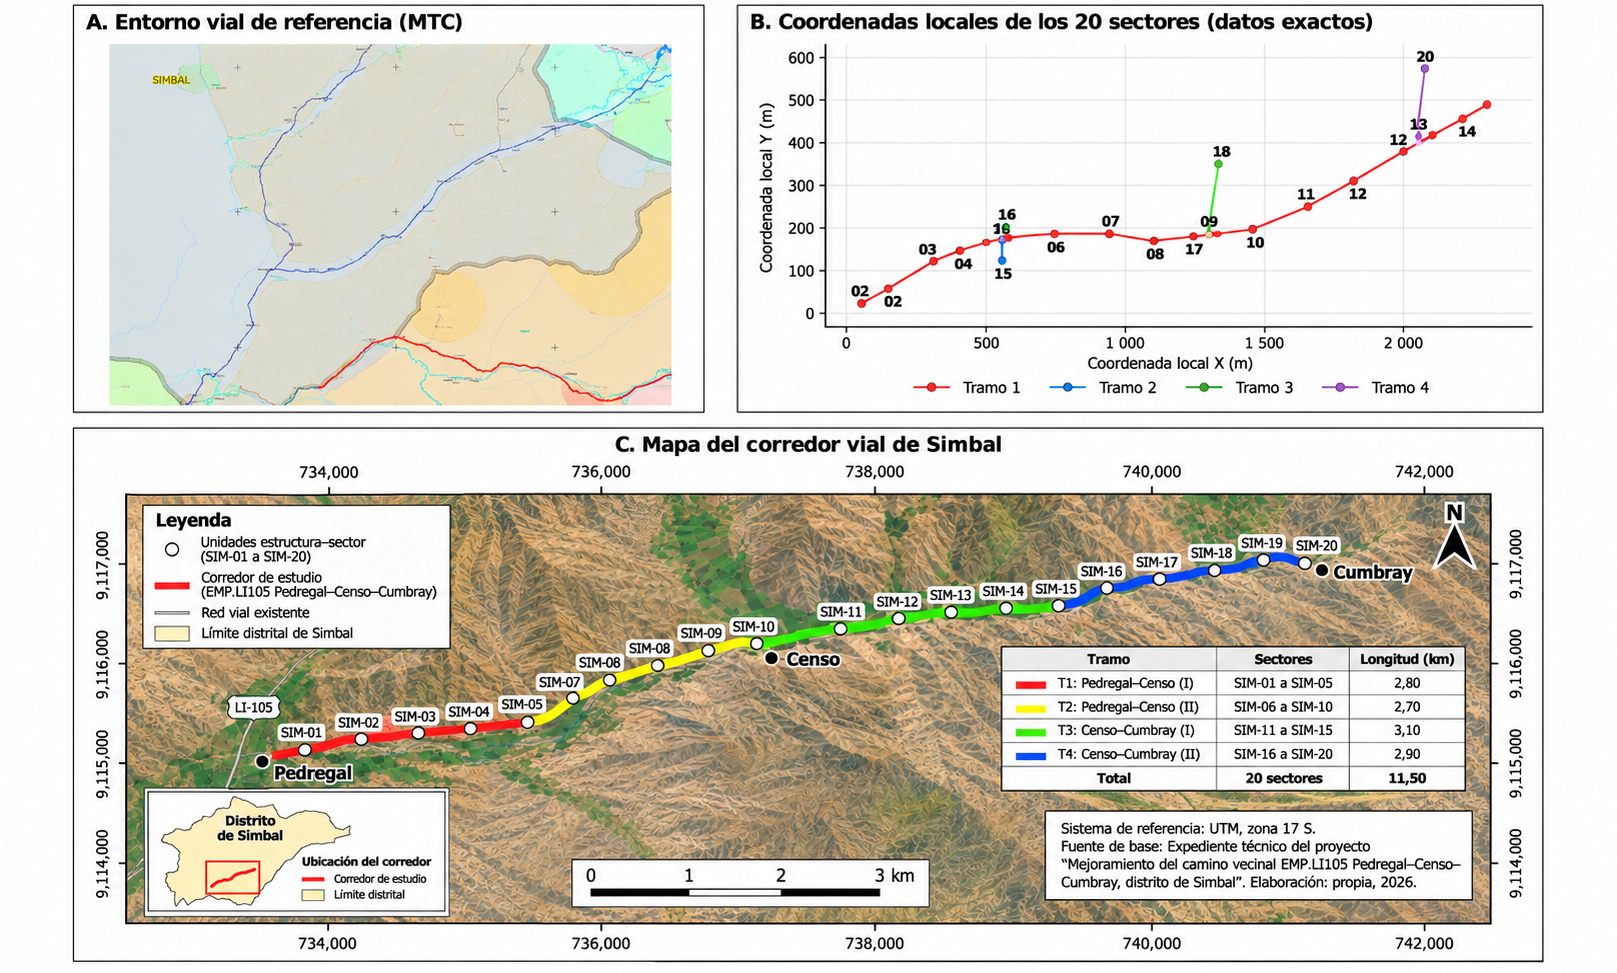
\includegraphics[width=0.96\linewidth,height=0.43\textheight,keepaspectratio]{figuras/Figura_05_Mapa_Compuesto_Simbal_2026.png}%
}{%
  \fbox{\parbox[c][4.5cm][c]{0.82\linewidth}{\centering
    Falta el archivo original de la Figura 5.\\[6pt]
    Copiar \texttt{Figura\_05\_Mapa\_Compuesto\_Simbal\_2026.png}\\
    a la carpeta \texttt{figuras/} sin modificarlo.}}%
}
\par
\notaTabla{El panel A presenta un entorno vial referencial; el panel B utiliza las coordenadas locales X--Y de la base Simbal 2026; el panel C representa cartográficamente el corredor.}
\end{figure}

La figura~\ref{fig:resultado-5} muestra en el panel B las veinte unidades estructura--sector agrupadas por tramo, mientras que los paneles A y C representan el entorno y el trazado vial; en correspondencia con la organización de los sectores, las coordenadas locales también sustentan la matriz de proximidad W utilizada en el análisis estadístico.

\subseccionTesis{Consolidación de los indicadores por unidad}

La descripción inicial por tramo constituye una clasificación de las unidades, no una agrupación adicional de mediciones. Cada identificador SIM conserva un único valor sectorial de CL, CT, PCI e IRI, aunque su construcción haya utilizado dos márgenes de drenaje, dos extremos transversales, varias subunidades de condición superficial y los recorridos longitudinales correspondientes; esta disposición mantiene constante el tamaño analítico de veinte pares para cada correlación.

Los cuatro indicadores obtenidos por unidad se reúnen en la tabla~\ref{tab:res-indicadores}, con identificación del tramo, progresiva y condición superficial de cada sector.

\tablaResultadoTres

La tabla~\ref{tab:res-indicadores} muestra variaciones de drenaje y pavimento entre las veinte unidades: SIM-17 concentra el menor CL (38,50 \%), el menor CT (61,71 \%), un PCI de 51,35 y el mayor IRI (4,7175 m/km), mientras que SIM-05 registra CL de 83,51 \%, CT de 84,40 \%, PCI de 82,01 e IRI de 1,9200 m/km. También es necesario considerar que los extremos de cada indicador se distribuyen entre sectores diferentes, puesto que el PCI mínimo corresponde a SIM-14, con 50,26, CL de 55,88 \%, CT de 71,94 \% e IRI de 4,2525 m/km, en tanto que el PCI máximo pertenece a SIM-02, con 83,39, CL de 83,47 \% y CT de 78,35 \%; adicionalmente, SIM-07 presenta el mayor CL, de 92,91 \%, y SIM-13 el mayor CT, de 91,26 \%, con lo cual la tabla permite reconocer valores extremos sin equiparar observaciones aisladas con una asociación general.

\subseccionTesis{Control de consistencia de la base consolidada}

La tabla~\ref{tab:res-auditoria} resume la conciliación aritmética de CL, CT, PCI e IRI y consigna las diferencias de longitud detectadas entre sector nominal y recorrido perfilado.

\tablaResultadoCuatro

La tabla~\ref{tab:res-auditoria} muestra diferencias nulas o cercanas a la precisión de máquina al reconstruir CL, CT, PCI e IRI a partir de los registros de las veinte unidades, con un máximo aproximado de \(1{,}42\times 10^{-14}\) en CT y \(4{,}44\times 10^{-16}\) en IRI, diferencias residuales respecto de los redondeos empleados para presentar los indicadores. Adicionalmente, el control de consistencia identifica divergencias entre longitud nominal y recorrido perfilado en SIM-14, SIM-16 y SIM-20, de 0,21 m, 0,11 m y 0,24 m, respectivamente; considerando lo anterior, la discrepancia mayor corresponde a SIM-20, cuya longitud nominal es 85,74 m frente a 85,50 m de perfilado, y se clasifica como diferencia entre registros de longitud, distinguiéndola del procedimiento de cálculo del IRI.

\seccionTesis{Resultados descriptivos de las variables de estudio}

\subseccionTesis{Condición del drenaje vial: continuidad longitudinal y abertura transversal}

Los estadísticos descriptivos de los cuatro indicadores se presentan en la tabla~\ref{tab:res-descriptivos} mediante media, desviación estándar, mediana, cuartiles y valores extremos, respetando la unidad de cada medición.

\tablaResultadoCinco

La tabla~\ref{tab:res-descriptivos} muestra medias de 71,07 \% para CL y 76,45 \% para CT, acompañadas por desviaciones estándar de 15,50 y 8,16 puntos porcentuales, respectivamente; de manera complementaria, las medianas fueron 72,45 \% para CL y 77,78 \% para CT, mientras que PCI registró 66,68 e IRI 3,1038 m/km. En este orden de ideas, la mayor desviación estándar de CL describe una variación más amplia de continuidad longitudinal entre los sectores, considerando las escalas porcentuales comunes de ambos indicadores de drenaje.

La figura~\ref{fig:resultado-6} presenta los diagramas de caja de CL y CT con una escala porcentual compartida, junto con las veinte observaciones individuales de cada indicador.

\begin{figure}[htbp]
\centering
\caption{Distribución de la continuidad longitudinal libre y de la abertura transversal libre}
\label{fig:resultado-6}
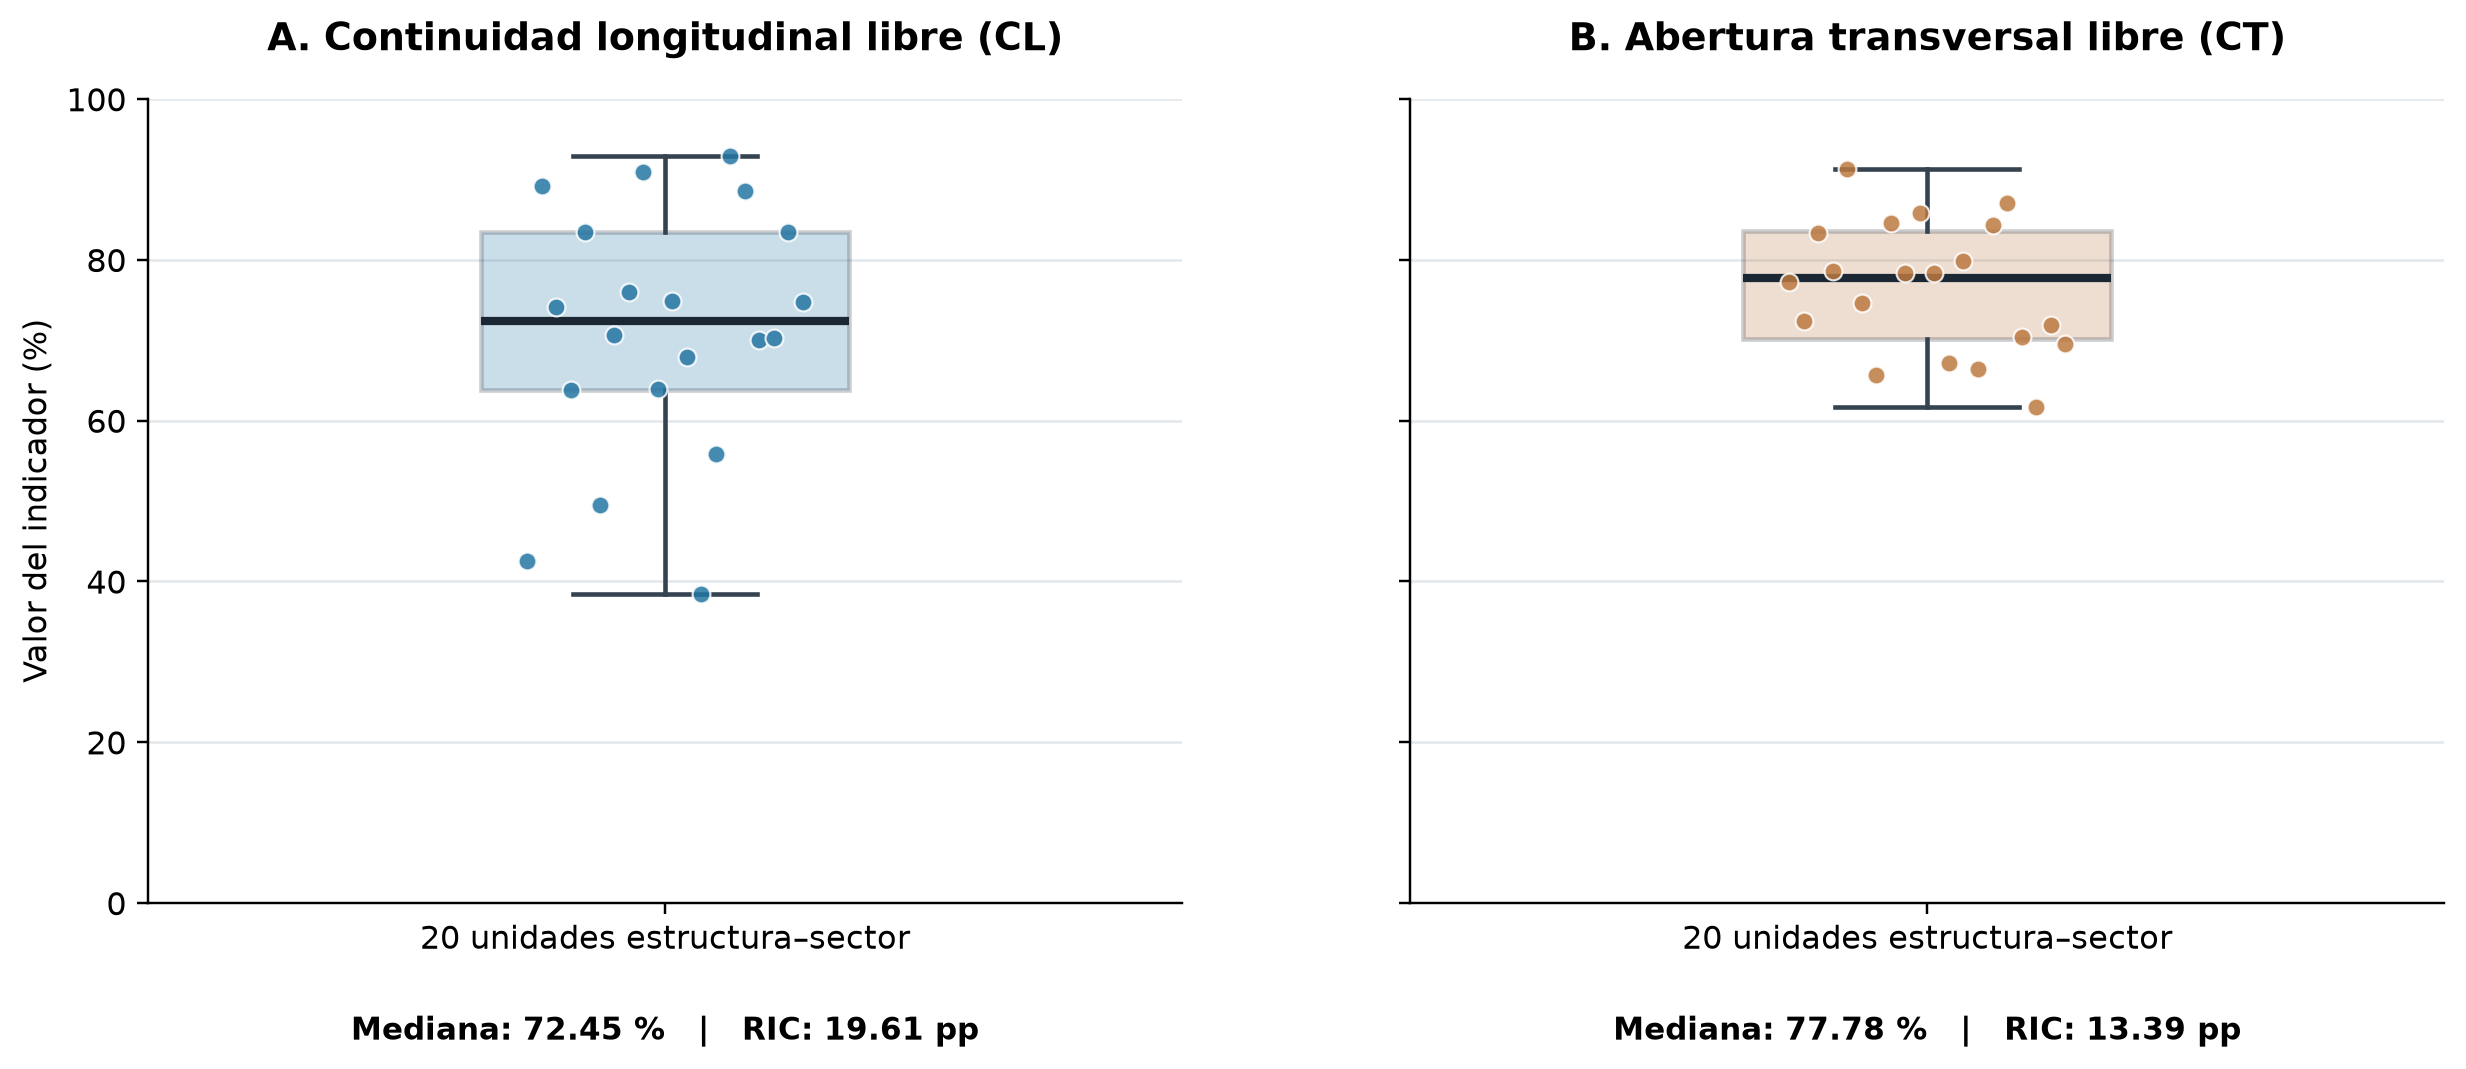
\includegraphics[width=0.94\linewidth,height=0.68\textheight,keepaspectratio]{figuras/Figura_06_CL_CT_sin_titulo_ni_nota.png}
\end{figure}

La figura~\ref{fig:resultado-6} muestra un rango intercuartílico de 19,61 puntos porcentuales para CL y de 13,39 para CT, por lo que la mitad central de los valores de CL ocupa un intervalo más amplio. Asimismo, los mínimos de 38,50 \% y 61,71 \%, respectivamente, se sitúan por debajo de sus medianas y completan la descripción de la dispersión observada en ambas dimensiones.

\subseccionTesis{Desempeño funcional del pavimento: PCI e IRI}

El desempeño funcional del pavimento se describió mediante PCI e IRI, indicadores que emplean escalas de lectura diferentes: los valores elevados de PCI corresponden a mejores condiciones superficiales, mientras que los valores elevados de IRI expresan mayor rugosidad. Sus estadísticas están reunidas en la tabla~\ref{tab:res-descriptivos} y su distribución individual se representa a continuación.

La figura~\ref{fig:resultado-7} representa las distribuciones de PCI e IRI en paneles independientes, porque el primero corresponde a una escala de cero a cien y el segundo a metros por kilómetro.

\begin{figure}[htbp]
\centering
\caption{Distribuciones del PCI y del IRI en los sectores de evaluación}
\label{fig:resultado-7}
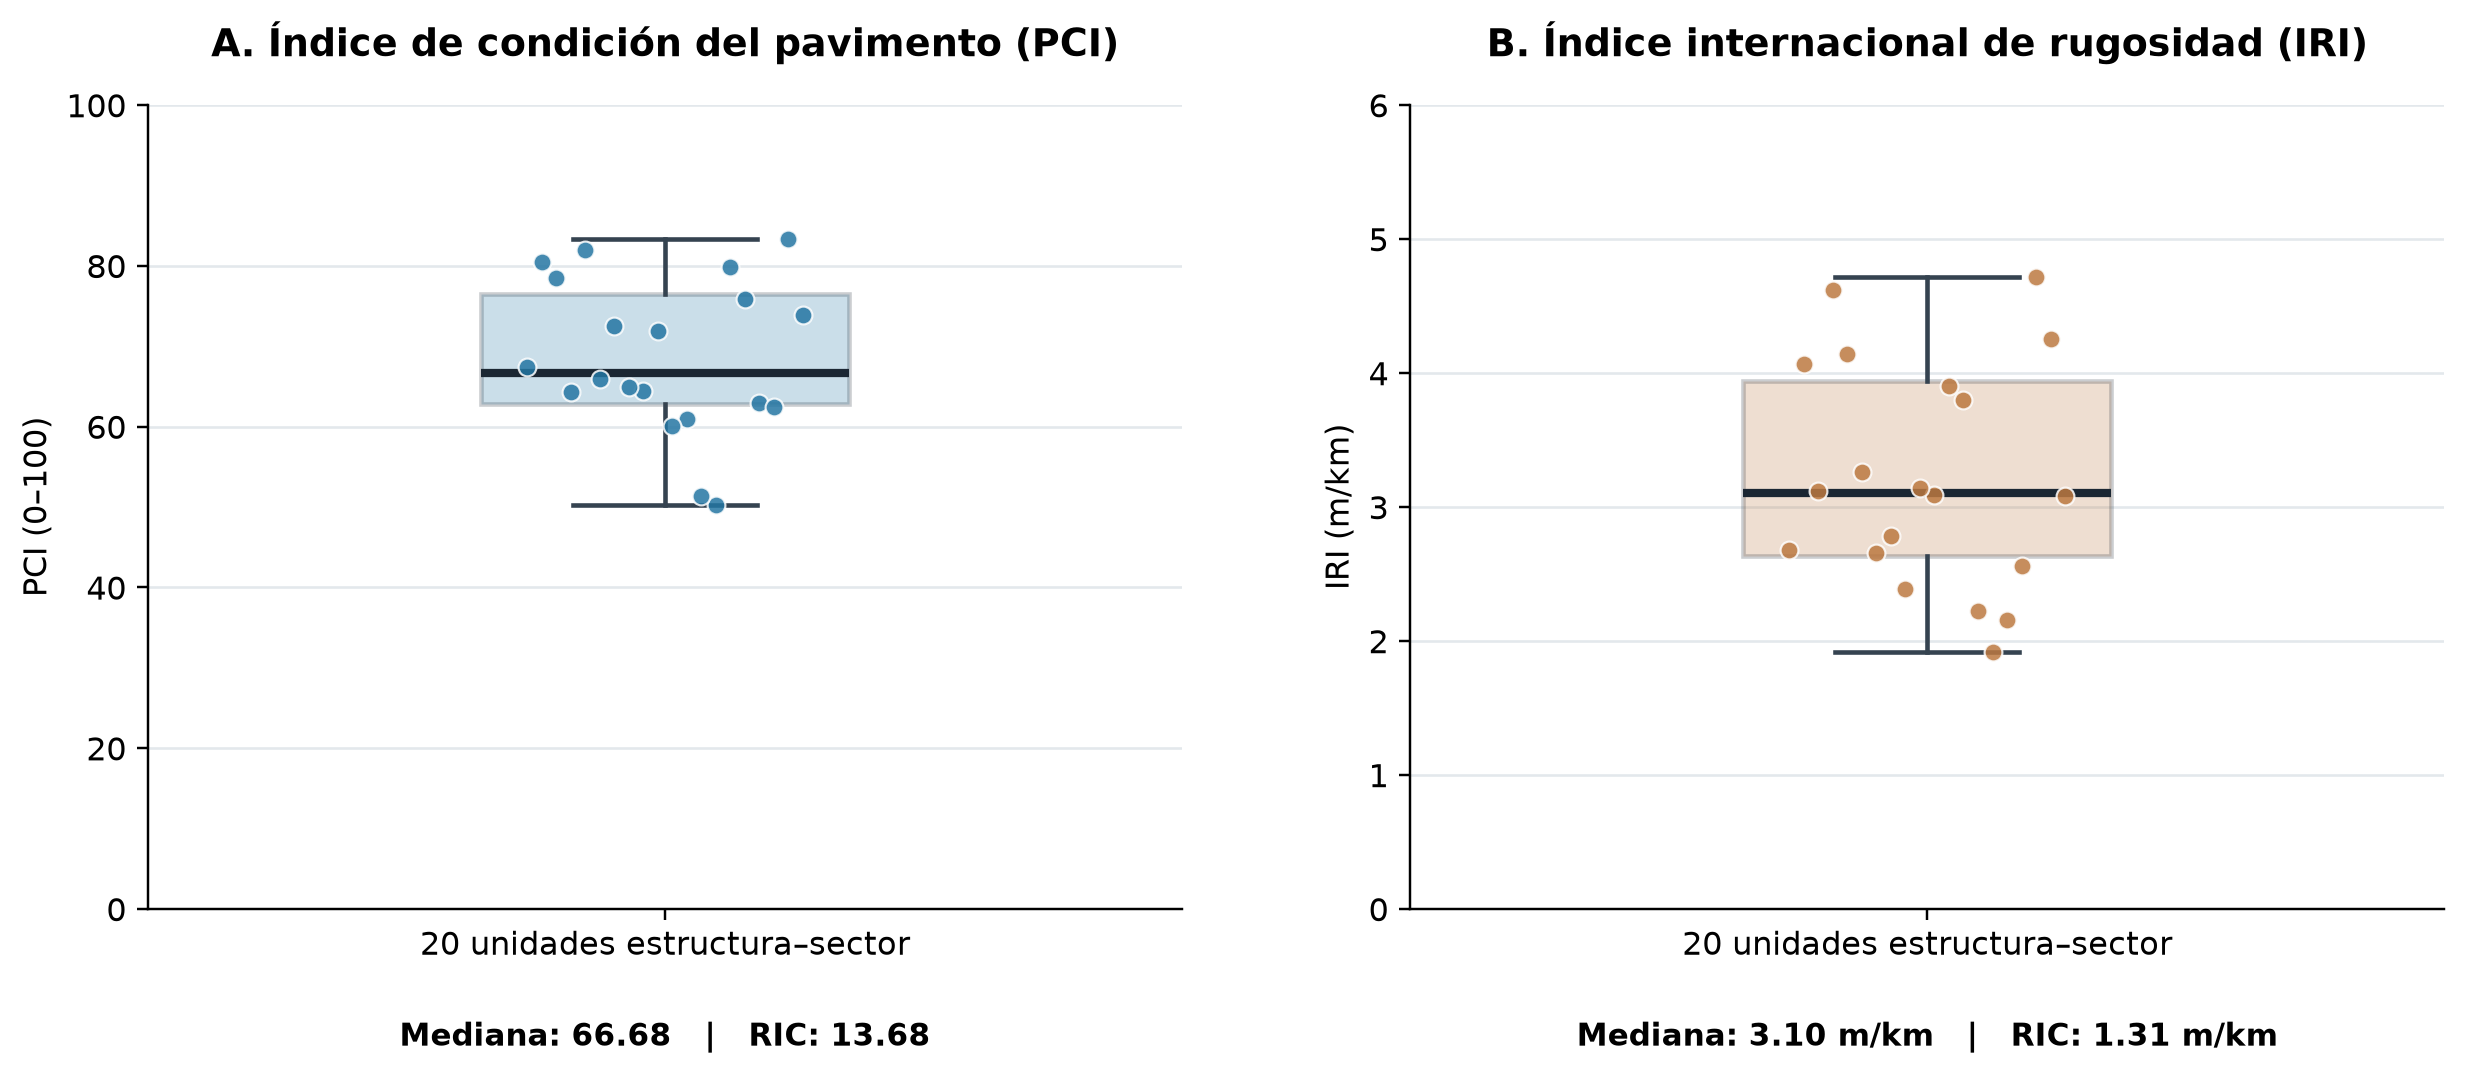
\includegraphics[width=0.94\linewidth,height=0.68\textheight,keepaspectratio]{figuras/Figura_07_Distribucion_PCI_IRI_Simbal_2026.png}
\end{figure}

La figura~\ref{fig:resultado-7} muestra que el PCI varía entre 50,26 y 83,39, con mediana de 66,68 y rango intercuartílico de 13,68 unidades, mientras que el IRI se distribuye entre 1,9200 y 4,7175 m/km, con mediana de 3,1038 m/km y rango intercuartílico de 1,31 m/km. En consecuencia, cada diagrama describe la variación interna de su propio indicador, sin que la altura de las cajas de ambos paneles constituya una comparación directa de magnitudes.

\subseccionTesis{Variabilidad descriptiva entre tramos}

La tabla~\ref{tab:res-promedios} desagrega los promedios de los cuatro indicadores por tramo, acompañados del número de unidades consideradas en cada agrupación.

\tablaResultadoSeis

La tabla~\ref{tab:res-promedios} muestra que el tramo 01, con catorce unidades, presenta medias de CL de 75,43 \%, CT de 77,63 \%, PCI de 70,39 e IRI de 3,0959 m/km, mientras que el tramo 02, integrado por dos unidades, registra 46,03 \%, 72,10 \%, 66,68 y 3,1713 m/km, respectivamente. Adicionalmente, los tramos 03 y 04, también con dos unidades cada uno, muestran valores diferenciados: el primero reúne medias de CL de 63,55 \%, CT de 72,50 \%, PCI de 63,60 e IRI de 3,9188 m/km, en tanto que el segundo alcanza 73,14 \%, 76,49 \%, 63,69 y 3,5225 m/km; de esta manera, la menor media de CL se identifica en el tramo 02 y el mayor IRI medio en el tramo 03, como descripciones de las agrupaciones y de sus tamaños de observación.

\seccionTesis{Relaciones observadas entre drenaje y desempeño funcional}

\subseccionTesis{Continuidad longitudinal y condición superficial (OE1/H1)}

La primera relación específica comparó la continuidad longitudinal libre con el índice de condición superficial del mismo sector. El ordenamiento de sus veinte pares permite describir la dirección de la correspondencia entre ambos indicadores sin sustituir el contraste espacial, presentado posteriormente.

La figura~\ref{fig:resultado-8} representa los veinte pares de CL y PCI por unidad, diferenciados por tramo e identificados mediante el código sectorial.

\begin{figure}[htbp]
\centering
\caption{Asociación entre continuidad longitudinal libre y PCI por unidad estructura–sector}
\label{fig:resultado-8}
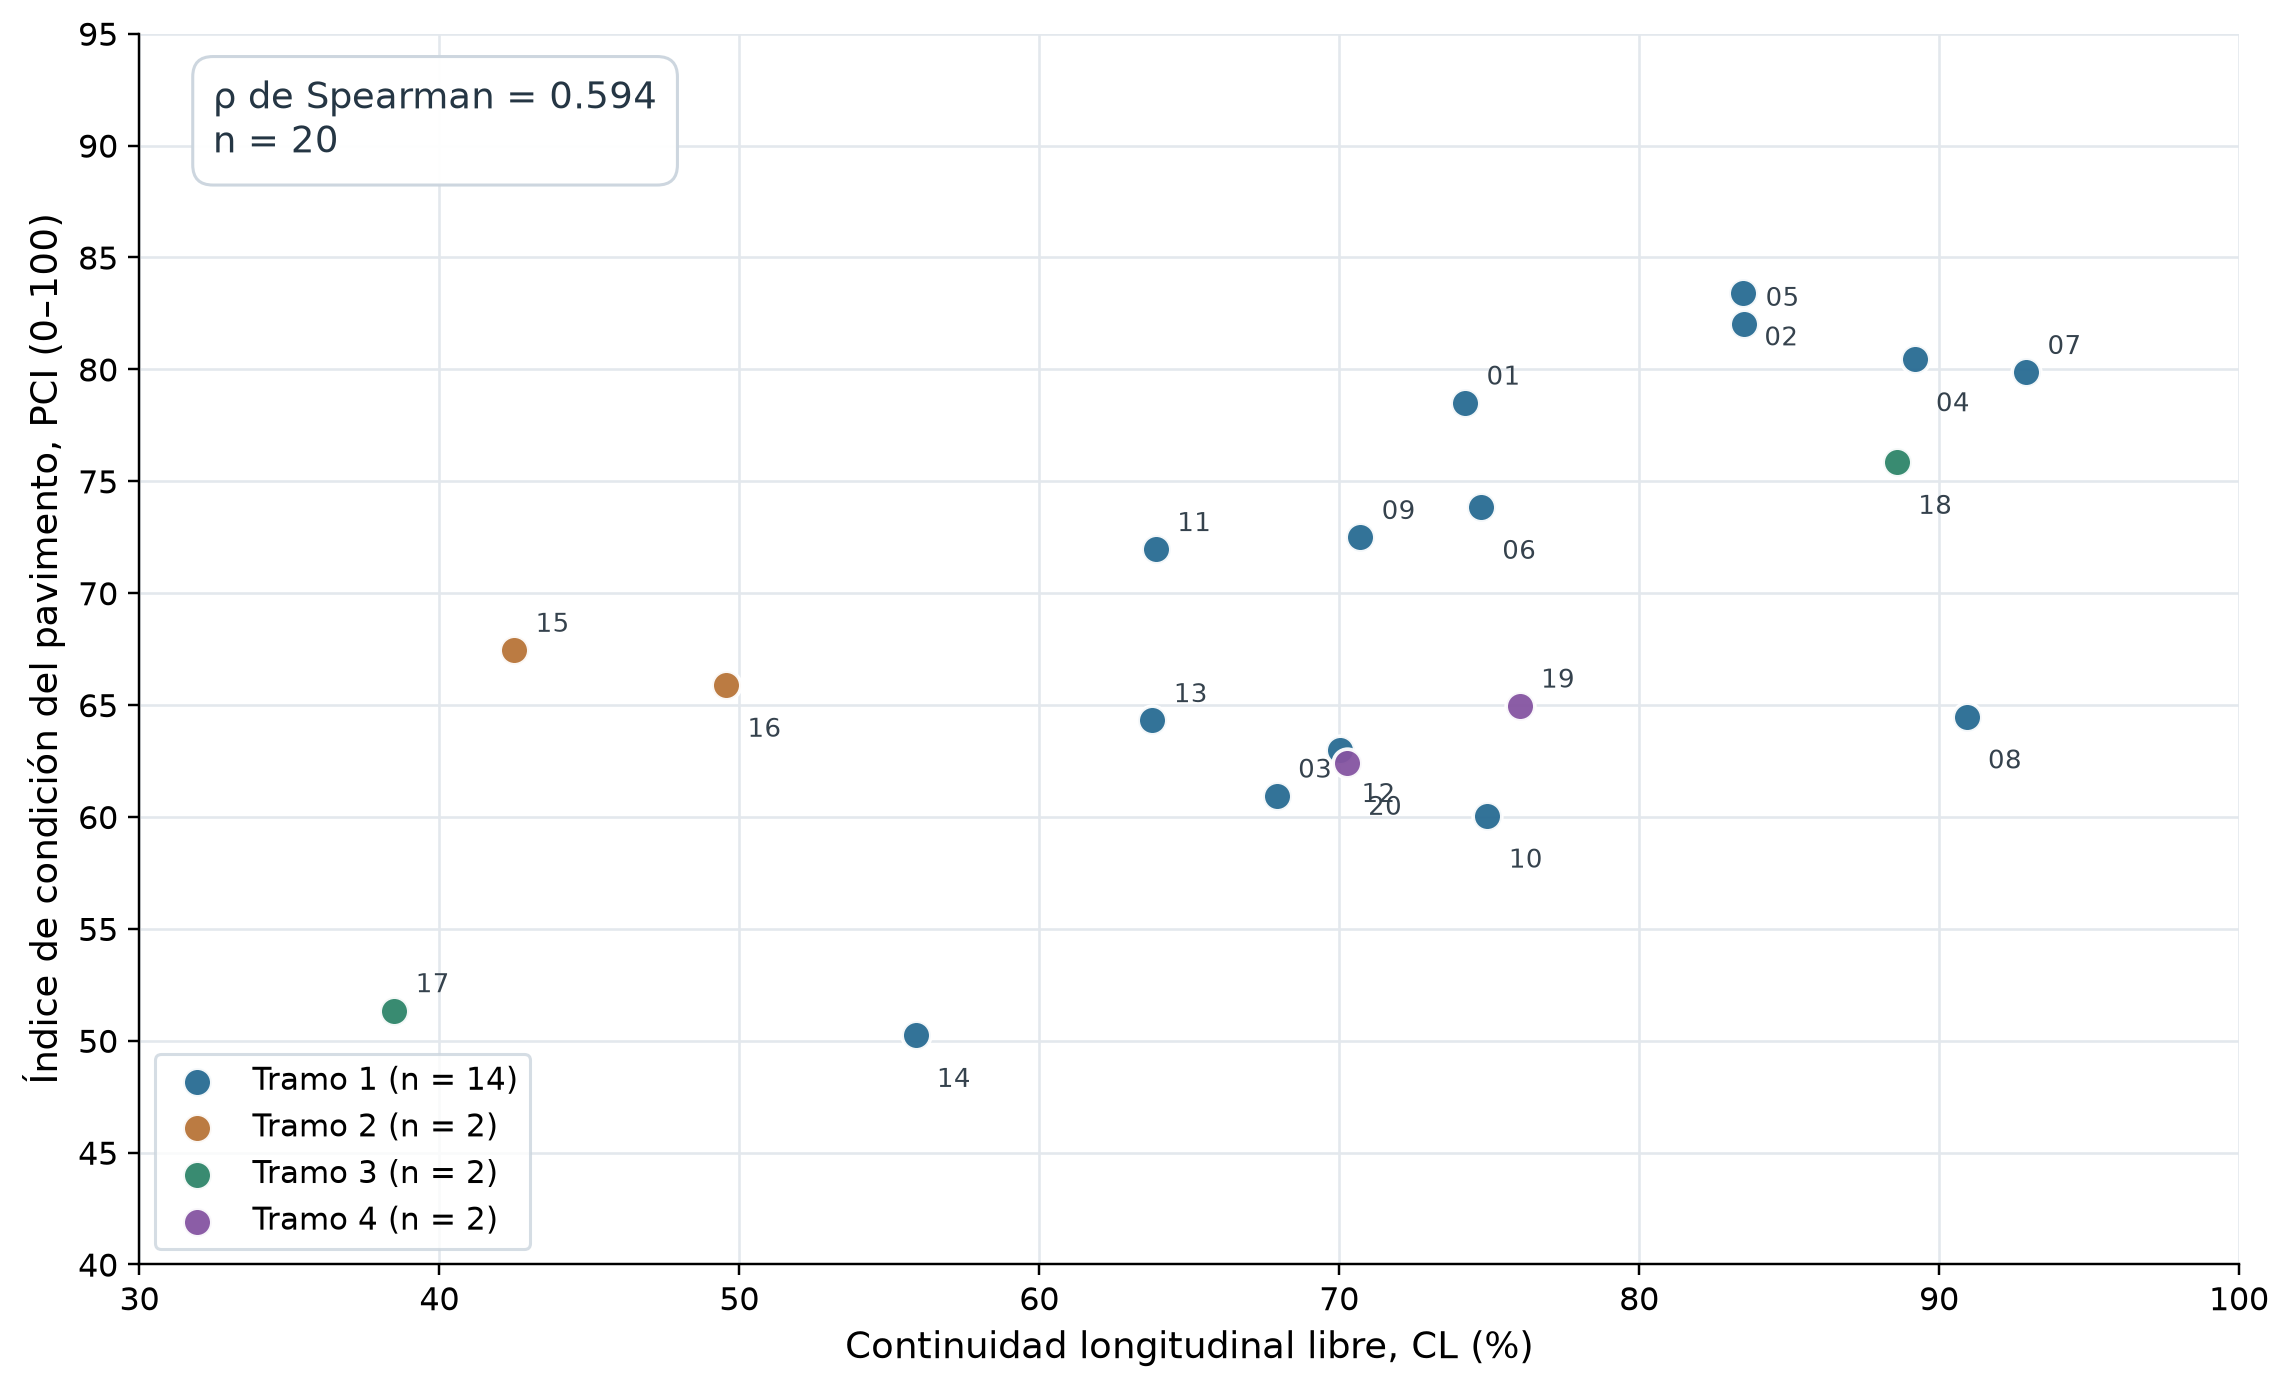
\includegraphics[width=0.94\linewidth,height=0.68\textheight,keepaspectratio]{figuras/Figura_08_Asociacion_CL_PCI_Simbal_2026.png}
\end{figure}

La figura~\ref{fig:resultado-8} muestra una disposición predominantemente ascendente de los puntos, congruente con el coeficiente de Spearman positivo de 0,5940. No todos los sectores siguen el mismo ordenamiento: SIM-08 registra CL de 90,92 \% con PCI próximo a 64,49, mientras que SIM-02 alcanza CL de 83,47 \% y PCI de 83,39; el resultado describe una asociación monotónica imperfecta entre los rangos de ambas mediciones.

\subseccionTesis{Continuidad longitudinal y rugosidad (OE2/H2)}

La segunda relación específica vinculó la continuidad longitudinal con la rugosidad del pavimento, conservando una medida porcentual para CL y una medida en m/km para IRI. La correlación por rangos examinó si la posición relativa de una unidad en la distribución de continuidad coincidía con su posición en la distribución de rugosidad.

La figura~\ref{fig:resultado-9} presenta la relación entre CL e IRI mediante los veinte pares sectoriales, utilizando porcentajes en el eje horizontal y m/km en el vertical.

\begin{figure}[htbp]
\centering
\caption{Asociación entre continuidad longitudinal libre e índice internacional de rugosidad}
\label{fig:resultado-9}
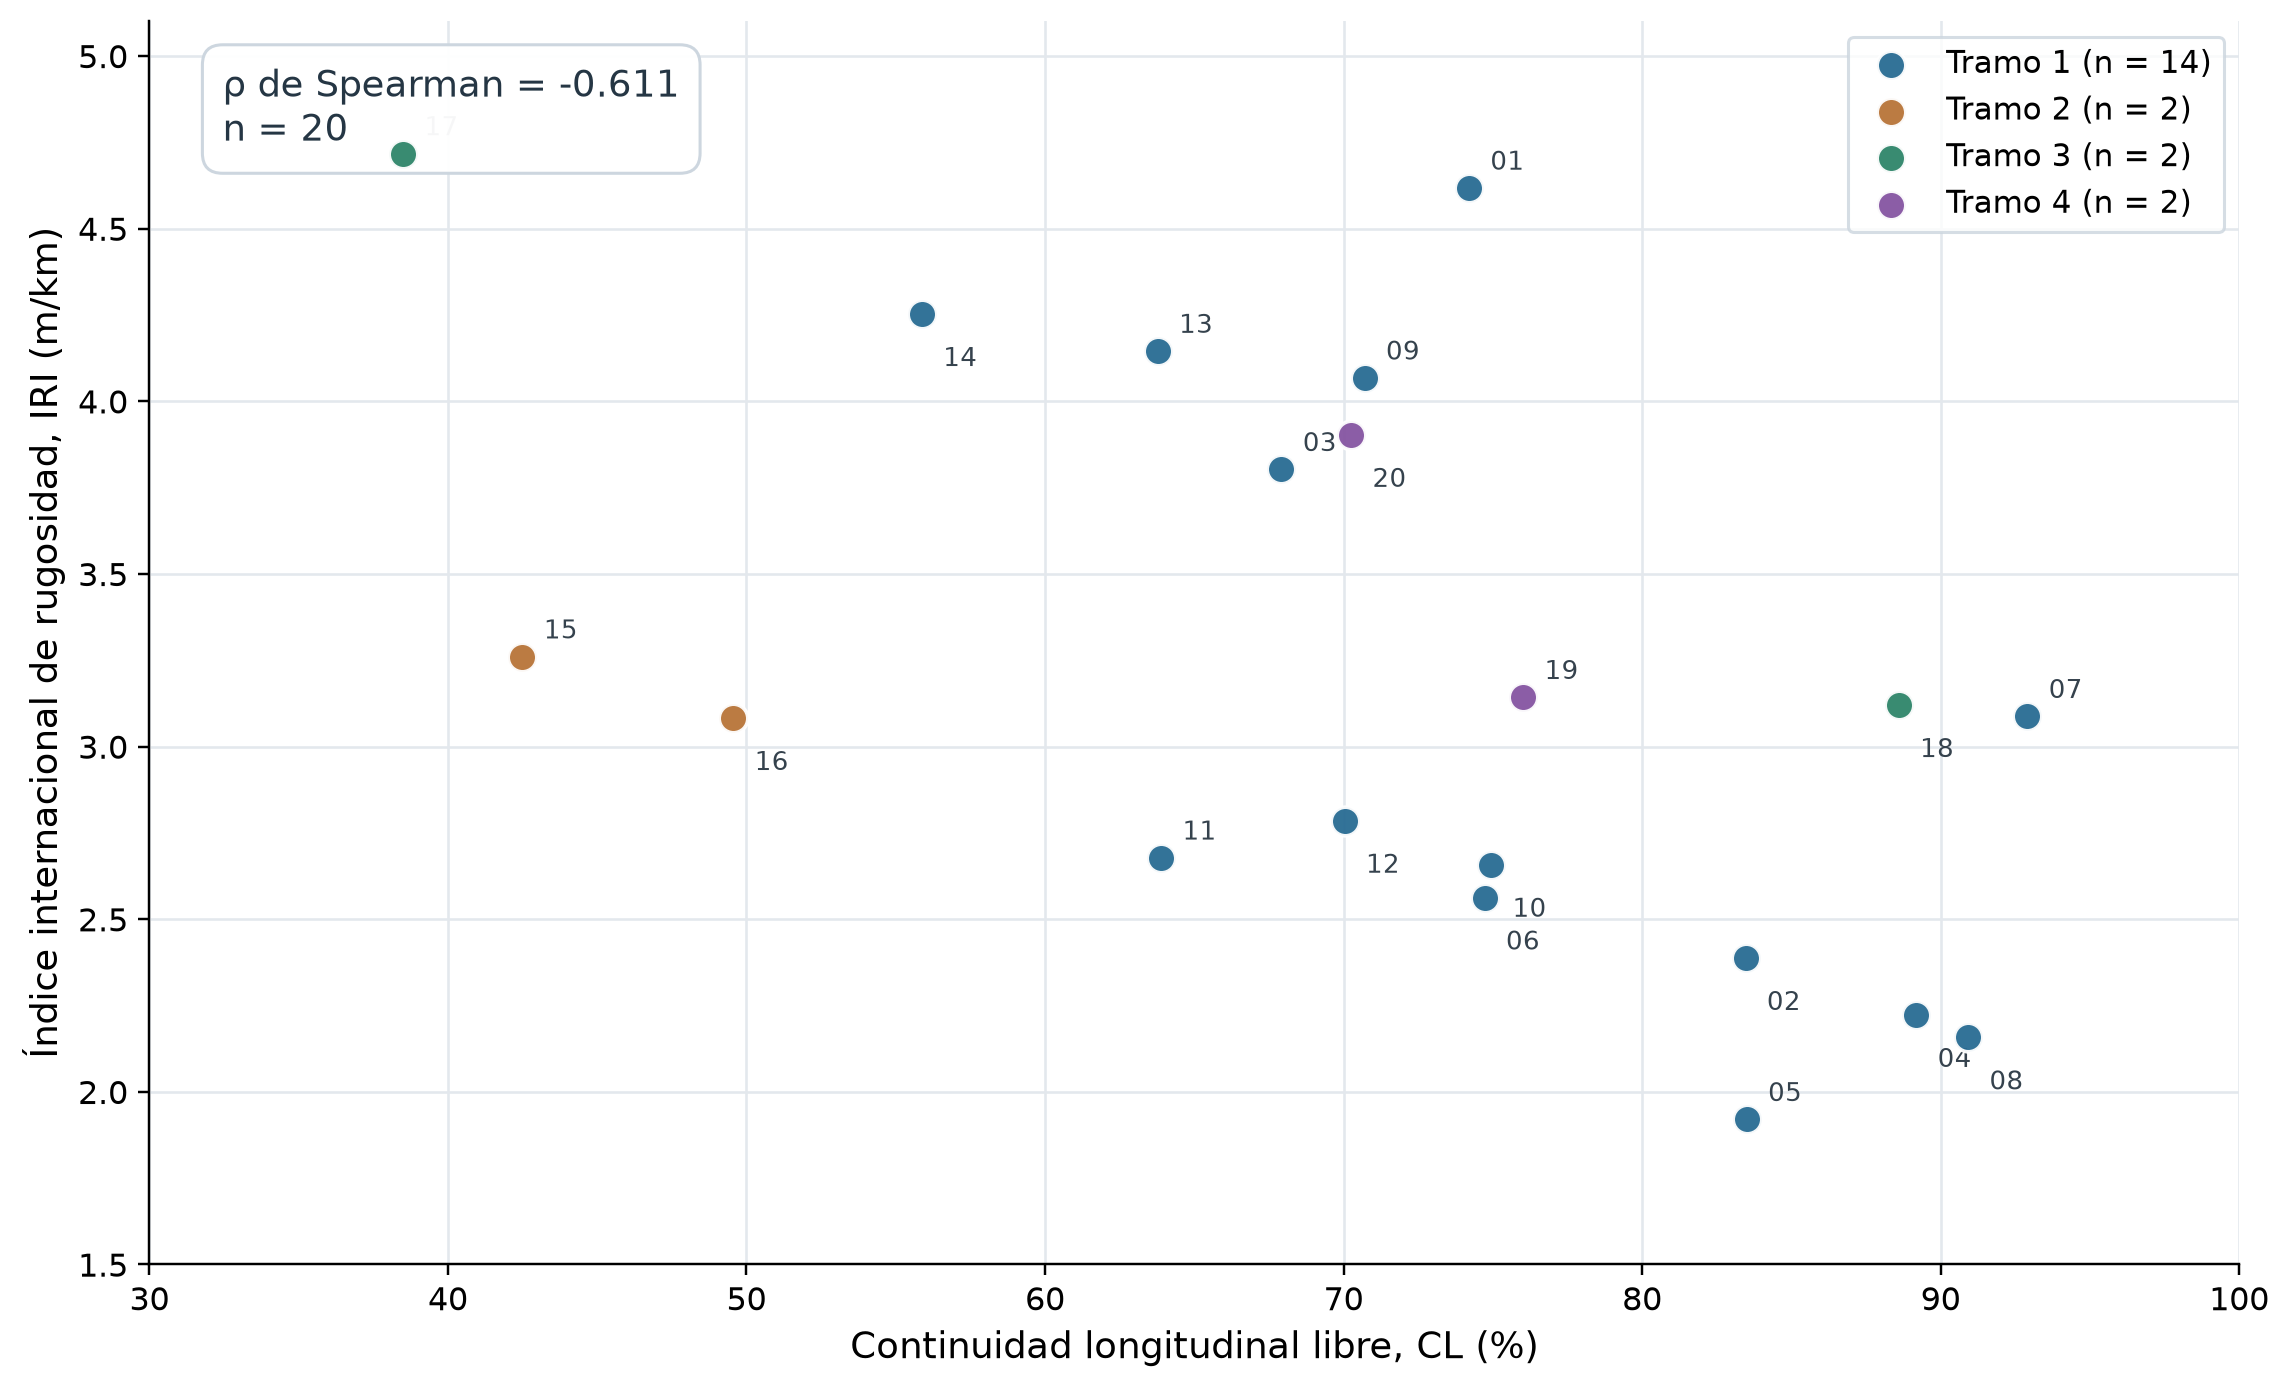
\includegraphics[width=0.94\linewidth,height=0.68\textheight,keepaspectratio]{figuras/Figura_09_Asociacion_CL_IRI_Simbal_2026.png}
\end{figure}

La figura~\ref{fig:resultado-9} muestra un ordenamiento predominantemente descendente, coherente con rho de Spearman de -0,6105. La dispersión incluye unidades con valores diferentes de IRI para porcentajes de CL cercanos; por ejemplo, SIM-01 combina CL de 74,20 \% con IRI de 4,6175 m/km y SIM-05 presenta CL de 83,51 \% con IRI de 1,9200 m/km, por lo que la correspondencia entre ambos indicadores no es exacta.

\subseccionTesis{Abertura transversal y condición superficial (OE3/H3)}

La tercera relación específica examinó la correspondencia entre el porcentaje de abertura transversal libre y la condición superficial del pavimento, utilizando los veinte pares sectoriales. A diferencia de la continuidad longitudinal, CT representa el porcentaje libre del extremo más restringido de cada pase, por lo que su lectura no debe confundirse con la continuidad de los márgenes.

La figura~\ref{fig:resultado-10} representa los pares de CT y PCI registrados en las veinte unidades, identificadas por tramo y código sectorial.

\begin{figure}[htbp]
\centering
\caption{Asociación entre abertura transversal libre y PCI por unidad estructura–sector}
\label{fig:resultado-10}
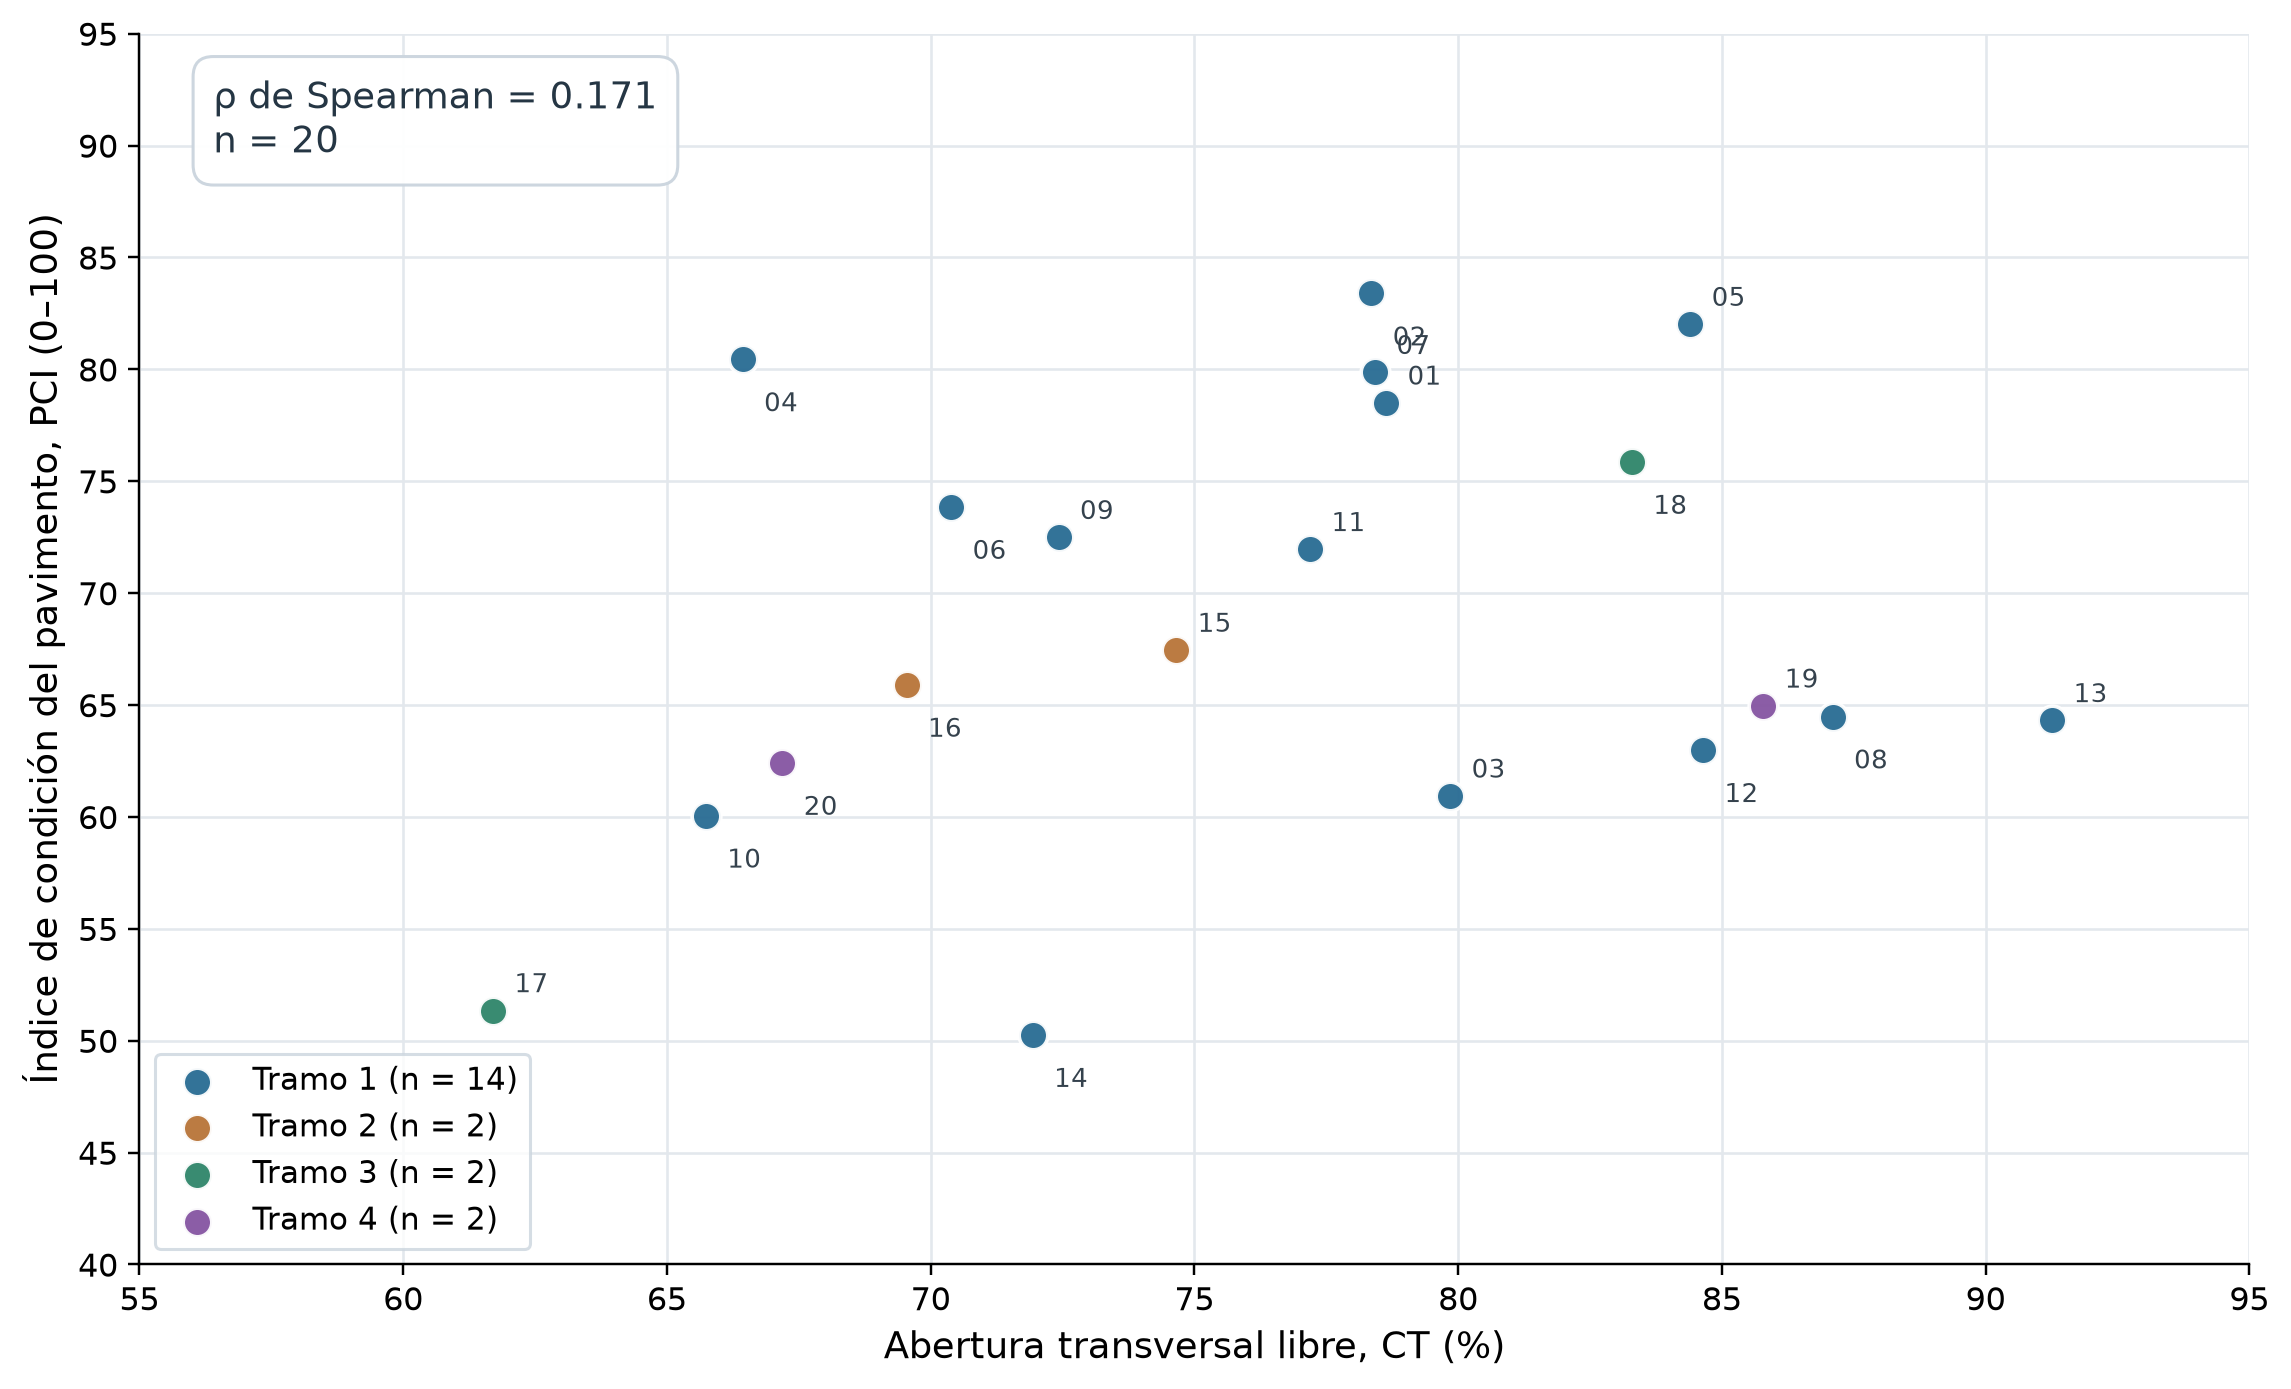
\includegraphics[width=0.94\linewidth,height=0.68\textheight,keepaspectratio]{figuras/Figura_10_Asociacion_CT_PCI_Simbal_2026.png}
\end{figure}

La figura~\ref{fig:resultado-10} muestra una nube de puntos dispersa a lo largo del intervalo de CT, con valores distintos de PCI para porcentajes semejantes de abertura transversal. El coeficiente de Spearman de 0,1714 resume esa correspondencia positiva de baja magnitud, sin una ordenación ascendente marcada de las veinte observaciones.

\subseccionTesis{Abertura transversal y rugosidad (OE4/H4)}

La cuarta relación específica reunió el porcentaje de abertura transversal libre y el índice de rugosidad longitudinal de cada sector. Como ambas mediciones proceden de instrumentos y escalas diferentes, la comparación se estableció sobre sus rangos y se describió mediante el coeficiente de Spearman.

La figura~\ref{fig:resultado-11} presenta la relación entre CT e IRI en un diagrama de dispersión que conserva las unidades originales de ambos indicadores.

\begin{figure}[htbp]
\centering
\caption{Asociación entre abertura transversal libre e índice internacional de rugosidad}
\label{fig:resultado-11}
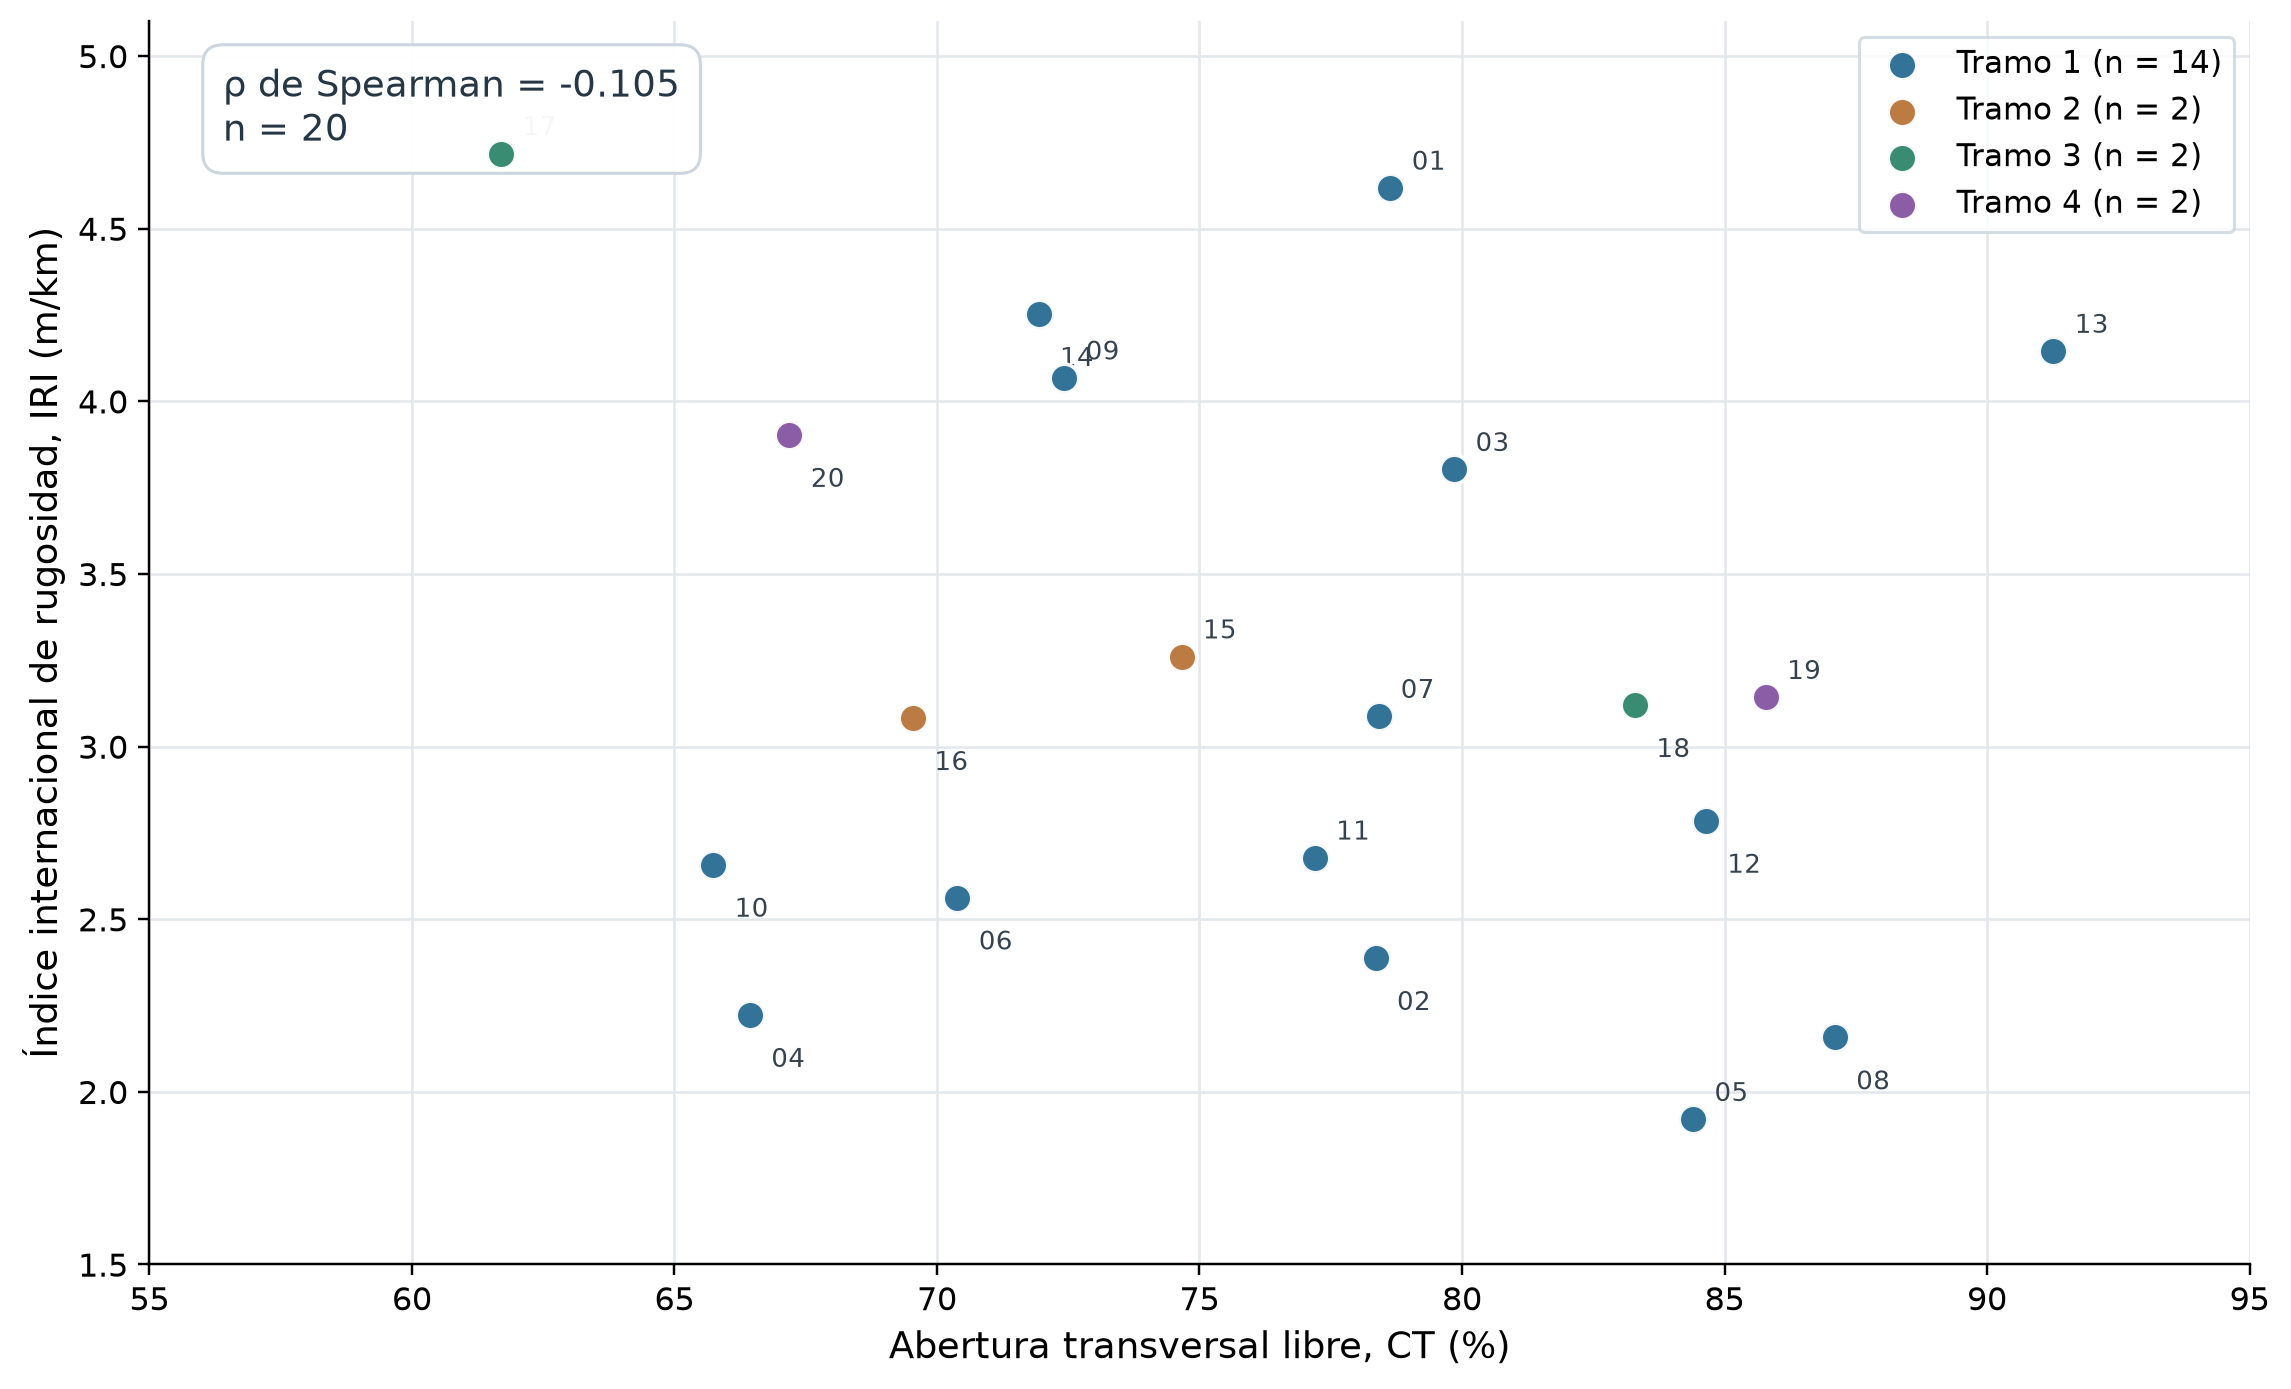
\includegraphics[width=0.94\linewidth,height=0.68\textheight,keepaspectratio]{figuras/Figura_11_Asociacion_CT_IRI_Simbal_2026.png}
\end{figure}

La figura~\ref{fig:resultado-11} muestra valores de IRI heterogéneos para los porcentajes de CT observados, sin una trayectoria descendente claramente definida. El coeficiente de Spearman de -0,1053 describe una asociación inversa de magnitud reducida, mientras que los sectores situados entre aproximadamente 65 \% y 85 \% de CT abarcan una parte amplia del intervalo de rugosidad registrado.

\subseccionTesis{Comparación preliminar de las cuatro relaciones}

Los cuatro diagramas representan pares formados en una misma unidad y mantienen sin transformar las unidades originales de los ejes. Las trayectorias visuales no se emplearon para obtener pendientes de regresión ni para expresar variación porcentual de PCI o IRI por cada punto de CL o CT; su función consistió en exponer el ordenamiento conjunto que sintetizan posteriormente los coeficientes de correlación por rangos.

La tabla~\ref{tab:res-spearman} reúne los cuatro coeficientes de Spearman convencionales, los valores p bilaterales y el número de pares válidos para comparar los contrastes antes del tratamiento espacial.

\tablaResultadoSiete

La tabla~\ref{tab:res-spearman} muestra correlaciones de CL con PCI (\(\rho\) = 0,5940; p = 0,00575) y con IRI (\(\rho\) = -0,6105; p = 0,00425), frente a asociaciones de menor magnitud para CT–PCI (\(\rho\) = 0,1714; p = 0,46989) y CT–IRI (\(\rho\) = -0,1053; p = 0,65873); considerando estos resultados convencionales, H1 y H2 registran valores p inferiores a 0,05, mientras que H3 y H4 superan ese umbral. En este orden de ideas, los cuatro coeficientes constituyen el punto de partida para los contrastes posteriores que incorporan el modelo nulo espacial y la corrección familiar de Holm.

\seccionTesis{Control espacial y contrastación inferencial de las hipótesis específicas}

La comparación convencional identifica un contraste entre la magnitud de las relaciones vinculadas con CL y las vinculadas con CT. Para CL, los coeficientes presentan magnitudes absolutas cercanas a seis décimas, pero con signos opuestos según el indicador funcional; para CT, ambos coeficientes son próximos a cero; este ordenamiento corresponde a las veinte unidades completas, por lo que todavía debe distinguirse de la correlación calculada sobre rangos residualizados después del tratamiento de las coordenadas espaciales.

\subseccionTesis{Matriz de vecindad y ajuste de tendencias espaciales}

Considerando las coordenadas métricas locales disponibles para cada sector, la configuración espacial se construyó mediante la selección de los dos vecinos euclidianos más próximos y la simetrización de las relaciones de vecindad; de esta manera, se obtuvo una matriz binaria de veinte filas y veinte columnas, sin autoconexiones, con veintiséis aristas no dirigidas. Esa estructura representa las conexiones de proximidad entre unidades y constituye la base de las aleatorizaciones espectrales de Moran utilizadas para evaluar las correlaciones.

La figura~\ref{fig:resultado-12} presenta la red estadística de vecindad construida sobre las coordenadas locales X e Y, con identificación de las veinte unidades.

\begin{figure}[htbp]
\centering
\caption{Red de vecindad espacial de las veinte unidades estructura–sector}
\label{fig:resultado-12}
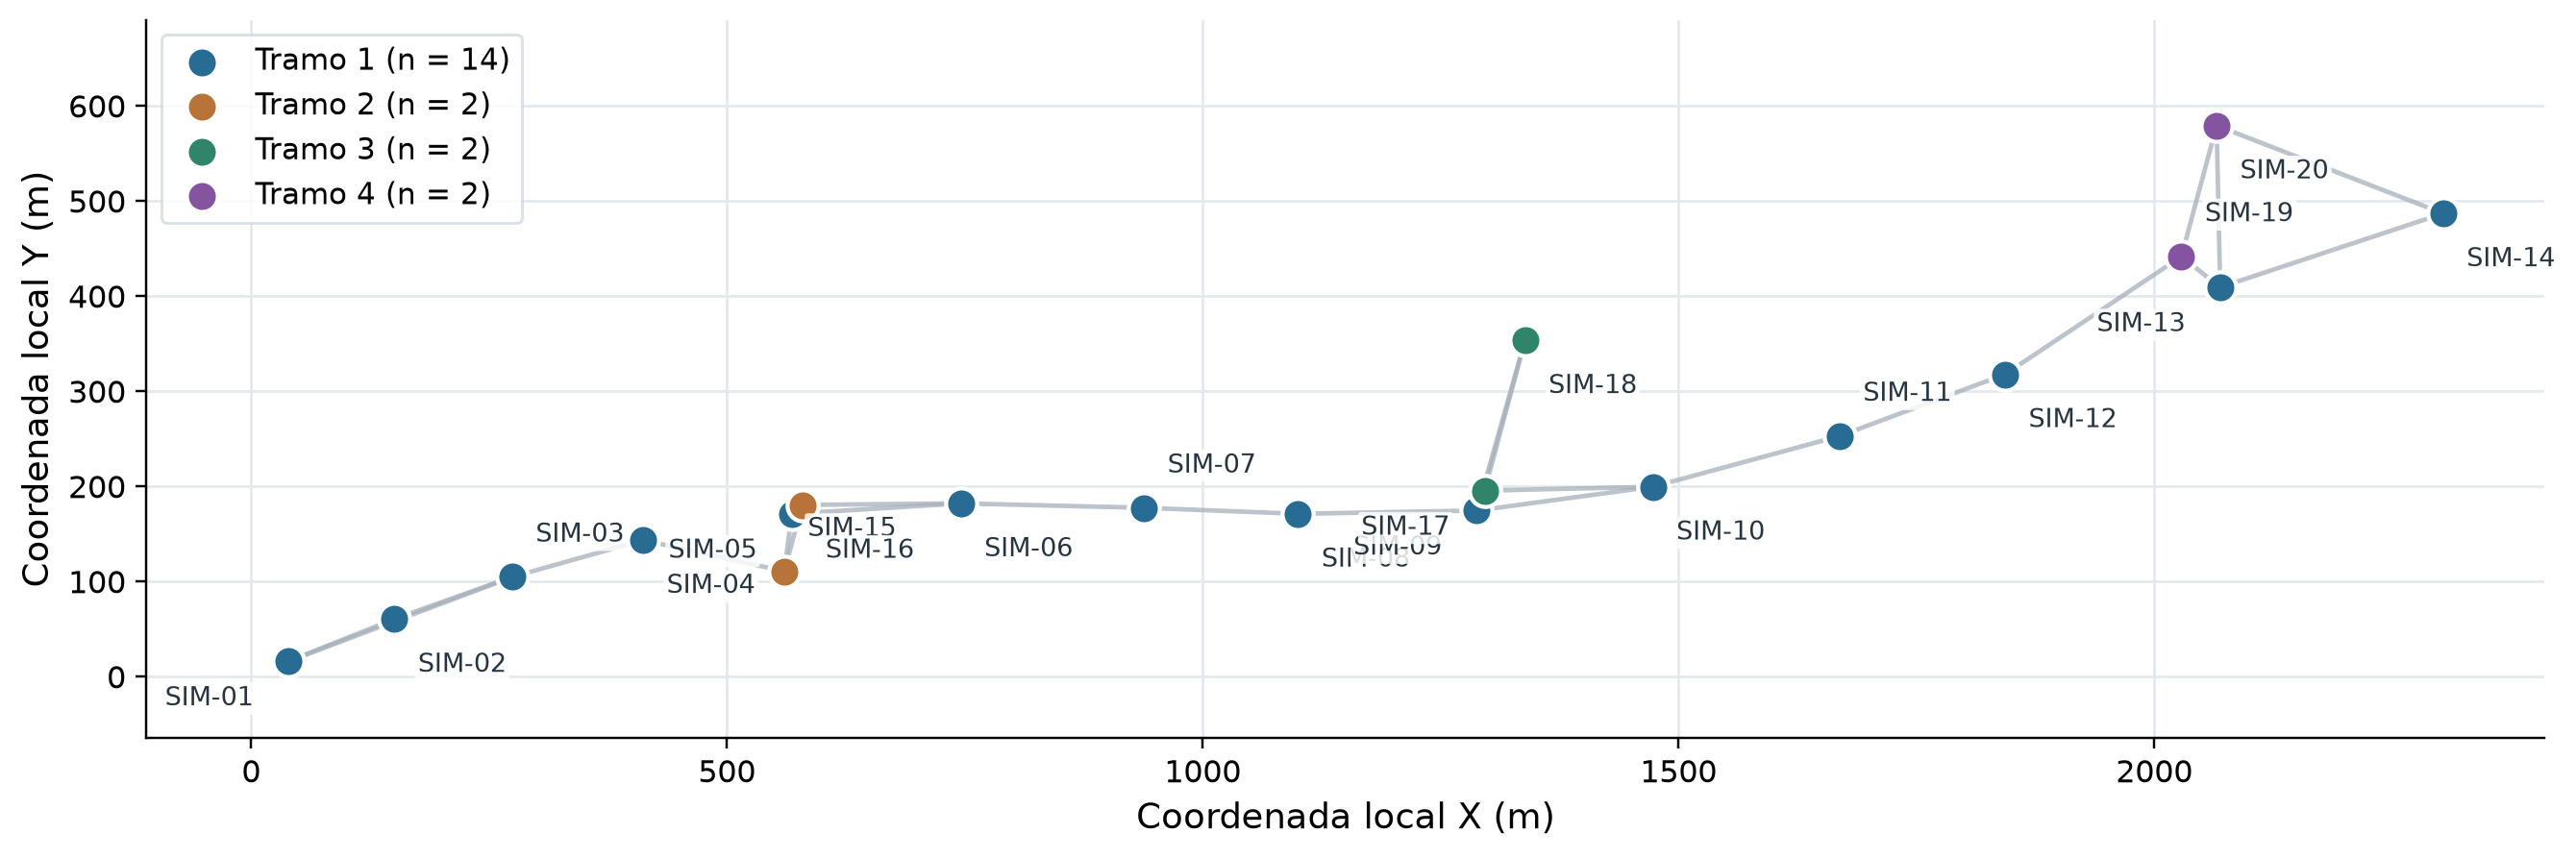
\includegraphics[width=0.94\linewidth,height=0.68\textheight,keepaspectratio]{figuras/Figura_12_Red_vecindad_espacial_Simbal_2026.png}
\end{figure}

La figura~\ref{fig:resultado-12} muestra 26 conexiones no dirigidas después de simetrizar la elección de los dos vecinos más próximos por unidad. El número de aristas incidente en cada punto no es uniforme porque la selección inicial de vecinos no siempre es recíproca; las líneas representan exclusivamente relaciones definidas en la matriz de pesos espaciales W.

Los coeficientes del ajuste lineal de rangos por coordenadas y los índices de Moran anteriores y posteriores a esa operación se presentan en la tabla~\ref{tab:res-moran-param}.

\tablaResultadoOcho

La tabla~\ref{tab:res-moran-param} muestra que los índices de Moran de los residuos fueron -0,1053 para CL, 0,0179 para CT, -0,3506 para PCI y -0,0691 para IRI. La mayor magnitud absoluta residual corresponde al PCI, mientras que CT presenta un valor próximo a cero; estas cifras describen la autocorrelación calculada bajo la matriz W y no constituyen por sí solas pruebas de significancia de esos índices.

\subseccionTesis{Aleatorización espectral de Moran y significancia espacial}

El control espacial se presenta después de las correlaciones convencionales porque requiere transformar previamente los indicadores en rangos y retirar su tendencia lineal respecto de las coordenadas locales X e Y; considerando esa transformación, la estructura de vecindad se utiliza para construir los contrastes espaciales de referencia. De esta manera, la magnitud examinada en esta etapa corresponde a una correlación entre residuos de rangos y se distingue del rho de Spearman presentado en la tabla~\ref{tab:res-spearman}, aunque ambos estadísticos informan sobre la dirección de las cuatro relaciones definidas.

Los cuatro contrastes espaciales se efectuaron sobre los rangos residualizados respecto de las coordenadas locales; para cada relación se consideraron 9 999 aleatorizaciones espectrales de Moran de la variable funcional residual, manteniendo fijo el vector del indicador de drenaje correspondiente. El estadístico observado se comparó bilateralmente con la distribución nula de su propia relación, conforme al procedimiento establecido en metodología.

La tabla~\ref{tab:res-moran-pruebas} presenta los coeficientes de correlación residualizada y el contraste bilateral obtenido mediante 9 999 aleatorizaciones por hipótesis, incluyendo el número de realizaciones tan extremas como el estadístico observado.

\tablaResultadoNueve

La tabla~\ref{tab:res-moran-pruebas} muestra que H1 registra 44 realizaciones extremas de 9 999 y p espacial de 0,0045, mientras que H2 contabiliza 355 y p de 0,0356. Para H3 y H4 se obtienen 2 674 y 5 216 realizaciones extremas, equivalentes a p de 0,2675 y 0,5217, respectivamente; se trata de valores de significancia individuales anteriores al ajuste de multiplicidad.

La figura~\ref{fig:resultado-13} presenta las cuatro distribuciones nulas obtenidas con la aleatorización espectral de Moran y señala el estadístico residualizado observado en cada contraste.

\begin{figure}[htbp]
\centering
\caption{Distribuciones nulas espaciales de H1, H2, H3 y H4 y ubicación de los estadísticos observados}
\label{fig:resultado-13}
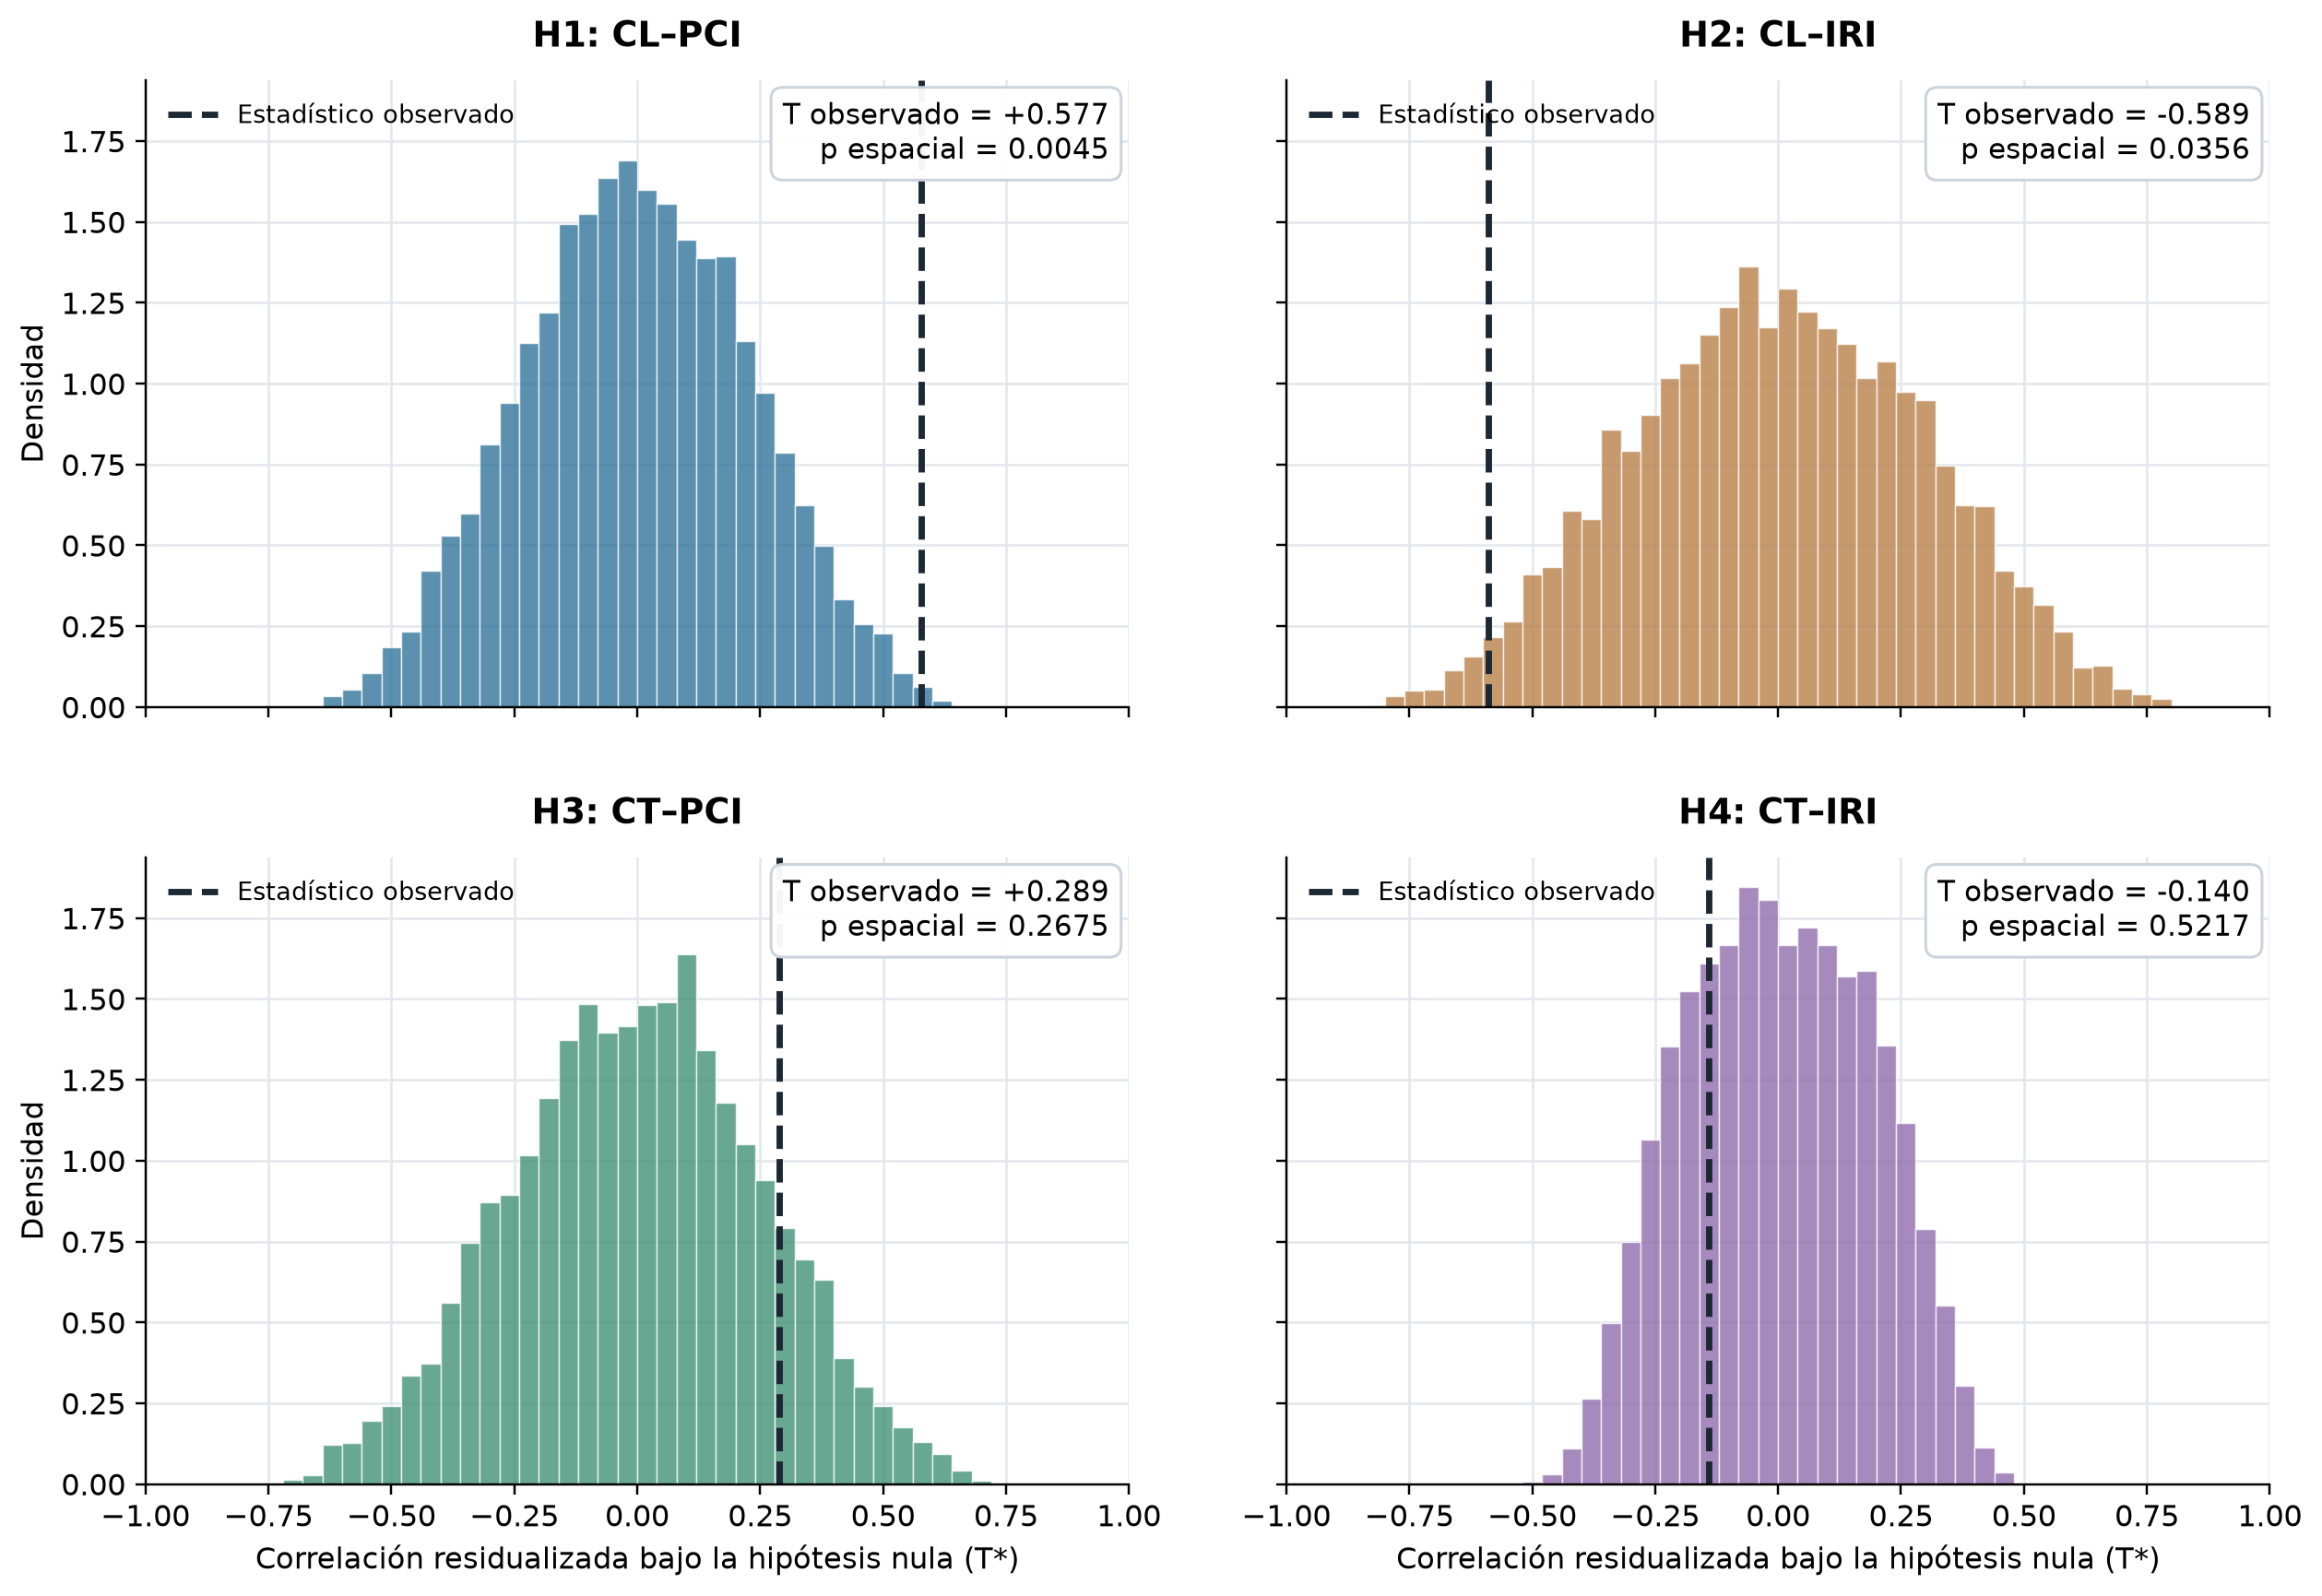
\includegraphics[width=0.94\linewidth,height=0.68\textheight,keepaspectratio]{figuras/Figura_13_Distribuciones_nulas_Moran_H1_H4_Simbal_2026.png}
\end{figure}

La figura~\ref{fig:resultado-13} muestra que los estadísticos observados de H1 (0,5773) y H2 (-0,5893) se sitúan en las zonas más alejadas del centro de sus distribuciones respectivas, en comparación con H3 (0,2893) y H4 (-0,1400). Esta posición corresponde a los diferentes conteos de realizaciones extremas consignados en la tabla~\ref{tab:res-moran-pruebas}, sin representar mediciones adicionales de los sectores.

La resolución numérica de la aleatorización se obtuvo mediante 9 999 realizaciones por contraste y la inclusión del estadístico observado en la regla de cálculo del valor p, conforme a la expresión establecida en metodología; en este orden de ideas, la tabla de contrastación conserva los conteos de realizaciones extremas que sustentan las probabilidades informadas. Para H1 se registraron 44 excedencias sobre un denominador de 10 000, mientras que H2, H3 y H4 presentan 355, 2 674 y 5 216, respectivamente; de esta manera, el procedimiento mantiene una regla de cómputo común para las cuatro relaciones analizadas.

\subseccionTesis{Corrección de Holm y decisión de las cuatro hipótesis específicas}

La tabla~\ref{tab:res-holm} presenta los valores p espaciales ordenados, sus factores de corrección, los valores ajustados mediante Holm y las decisiones con un nivel familiar de significancia de 0,05.

\tablaResultadoDiez

La tabla~\ref{tab:res-holm} muestra que H1 registra p ajustado de 0,0180, inferior a 0,05, por lo que cumple el criterio de significancia familiar. H2 obtiene 0,1068 y H3 y H4, 0,5350 cada una, valores superiores al umbral; así, la única decisión afirmativa se refiere a CL–PCI, sin que la falta de significancia de las otras asociaciones equivalga a demostrar coeficientes poblacionales exactamente nulos.

La figura~\ref{fig:resultado-14} representa gráficamente los cuatro valores p ajustados por Holm frente al umbral común de 0,05.

\begin{figure}[htbp]
\centering
\caption{Valores p ajustados por Holm y umbral de significancia familiar}
\label{fig:resultado-14}
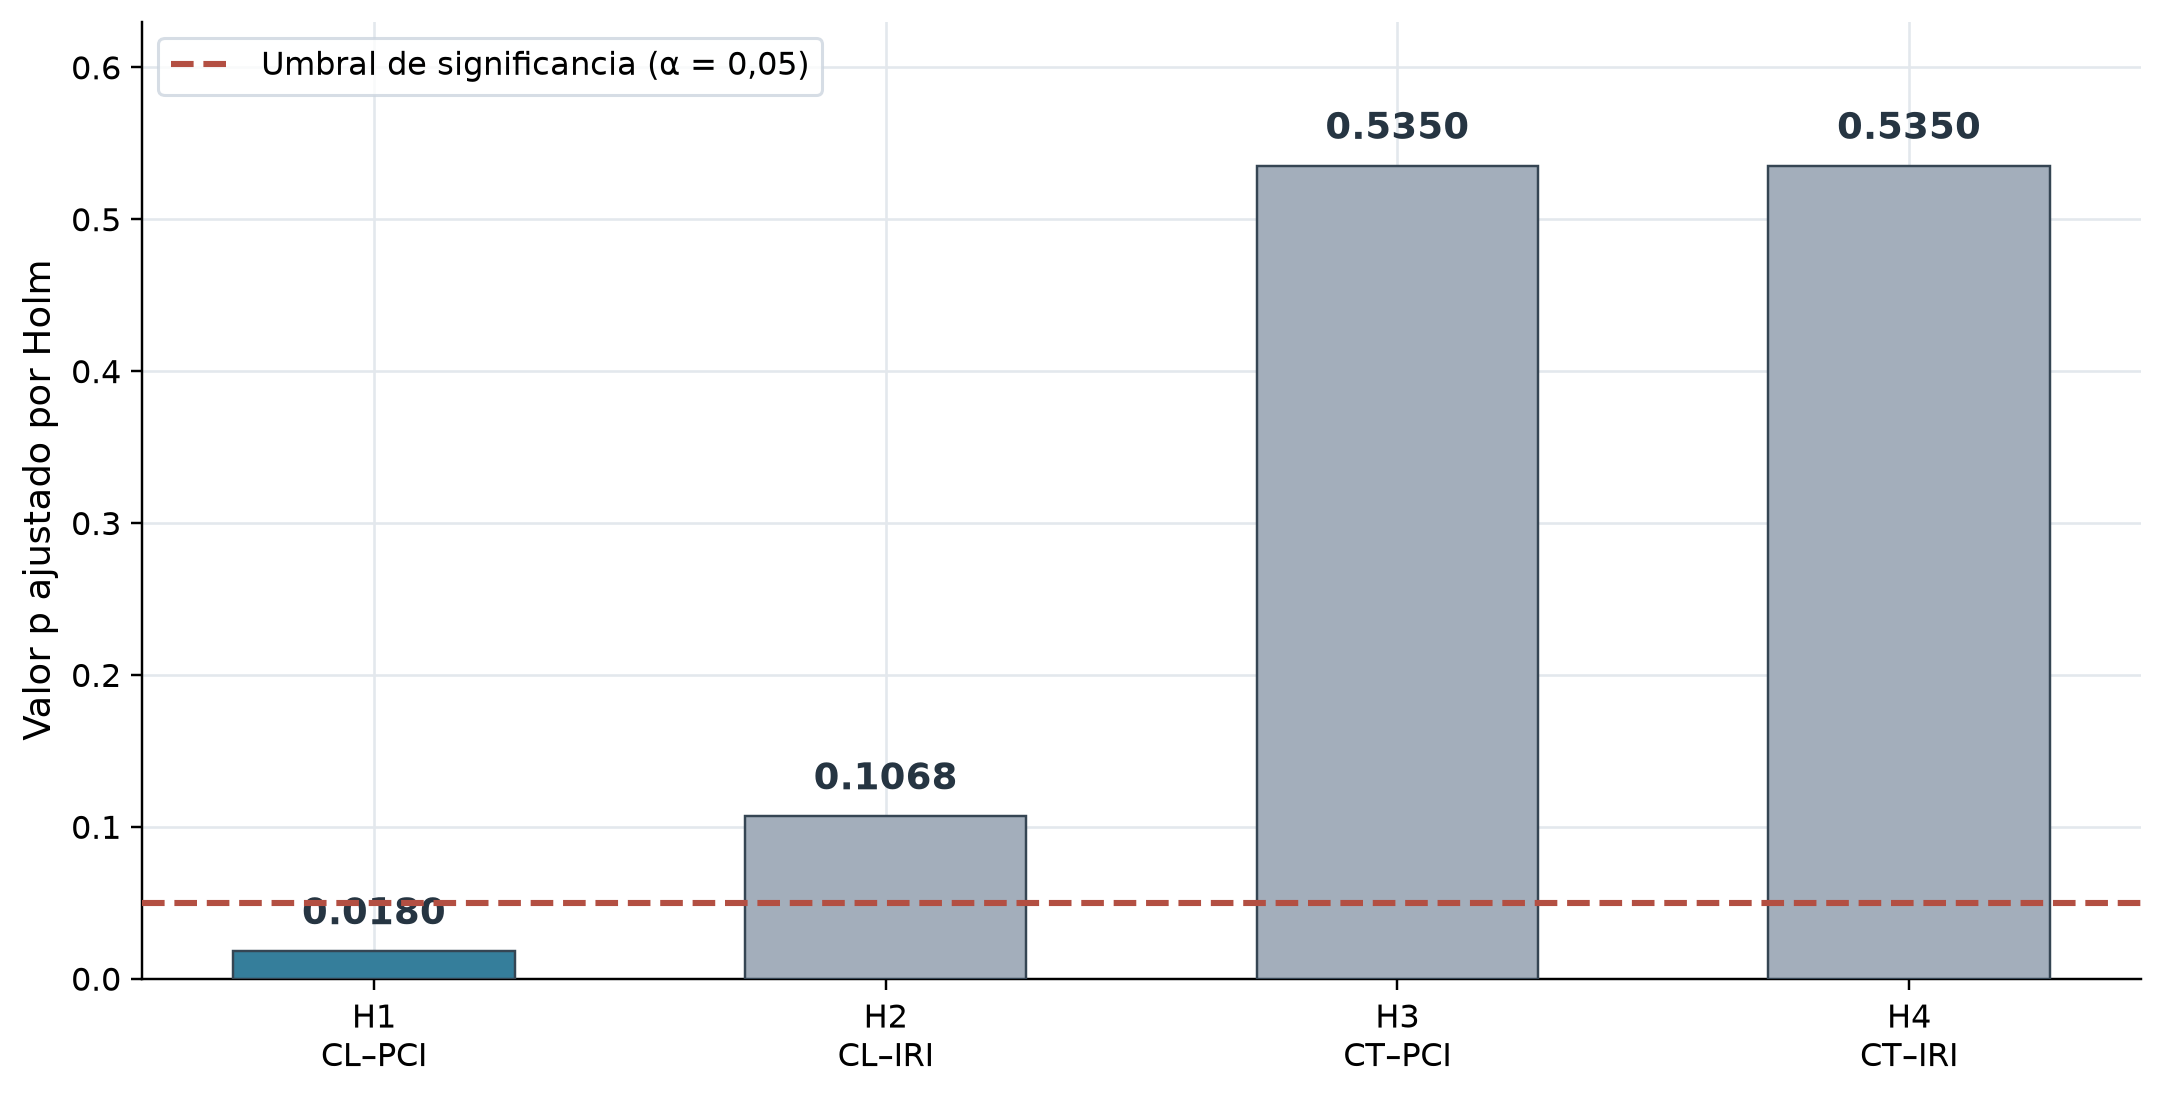
\includegraphics[width=0.94\linewidth,height=0.68\textheight,keepaspectratio]{figuras/Figura_14_Valores_p_Holm_Simbal_2026.png}
\end{figure}

La figura~\ref{fig:resultado-14} muestra que la barra de H1 queda por debajo de la línea de significancia, mientras que H2, H3 y H4 la superan. La diferencia visual reproduce los valores ajustados de la tabla~\ref{tab:res-holm} y señala una sola relación estadísticamente significativa dentro de la familia de contrastes evaluada.

\subseccionTesis{Sensibilidad de las correlaciones a la exclusión de unidades}

La tabla~\ref{tab:res-loo} presenta el mínimo y el máximo de las veinte correlaciones recalculadas para cada hipótesis al excluir sucesivamente una de las unidades.

\tablaResultadoOnce

La tabla~\ref{tab:res-loo} muestra que H1 mantiene correlaciones entre 0,5316 y 0,6807, H2 entre -0,6789 y -0,5456, y H3 entre 0,0439 y 0,2684; en estos tres casos el signo no cambia al retirar una unidad. En H4 el intervalo varía de -0,2211 a 0,0439 e incluye valores positivos, por lo que el signo de la correlación no se conserva en todas las exclusiones; el diagnóstico describe estabilidad de rho, no significancia estadística.

\seccionTesis{Contrastación de la hipótesis general}

La hipótesis general postuló una relación entre la condición del drenaje vial y el desempeño funcional del pavimento, operacionalizados mediante dos indicadores por variable. El proyecto no definió un índice compuesto ni un estadístico global que integrara CL y CT, por un lado, y PCI e IRI, por otro; por ello, la evaluación se efectuó a partir de la lectura conjunta de las cuatro hipótesis específicas, sin calcular una correlación adicional entre variables agregadas que no estuviera prevista en la matriz de operacionalización.

El resultado principal corresponde al respaldo estadístico de H1, para CL–PCI, con correlación espacial ajustada de 0,5773 y p de Holm de 0,0180; adicionalmente, CL–IRI mostró un coeficiente inverso de -0,5893, aunque su p corregido alcanzó 0,1068, mientras que CT–PCI y CT–IRI registraron 0,5350 en ambos casos. Considerando lo anterior, el patrón inferencial se concentra en una asociación significativa específica y tres relaciones que superan el umbral familiar establecido, por lo que la interpretación conjunta se organiza mediante las decisiones individuales de las cuatro hipótesis.

La interpretación de la hipótesis general permaneció delimitada a ese patrón de resultados. Se identificó una asociación significativa en una de las cuatro relaciones definidas, mientras que las otras tres no cumplieron el criterio familiar de decisión; de este modo, no correspondió declarar respaldada integralmente la hipótesis general mediante la sola existencia de un contraste específico favorable; esta conclusión conserva la distinción entre una evidencia parcial de asociación y una demostración global de relación, distinción necesaria para no sustituir por una apreciación narrativa la ausencia de una prueba compuesta previamente operacionalizada.

\seccionTesis{Síntesis de resultados por objetivos e hipótesis}

La clasificación de los cuatro contrastes constituye la información utilizada para examinar la proposición general. H1 presenta un coeficiente residual positivo y un valor de significancia ajustado inferior al límite familiar; H2 presenta un coeficiente residual negativo de magnitud comparable, pero una significancia corregida superior al límite, mientras que H3 y H4 muestran coeficientes de menor magnitud absoluta; la exposición conjunta conserva estas diferencias sin asignarles pesos iguales, convertirlas en un promedio de correlaciones ni formular un criterio global que no fue operacionalizado en el proyecto.

La tabla~\ref{tab:res-sintesis} reúne los resultados por objetivo específico e hipótesis, utilizando los coeficientes residualizados, los valores p espaciales y los valores ajustados de Holm.

\tablaResultadoDoce

La tabla~\ref{tab:res-sintesis} muestra una relación con significancia familiar: OE1/H1, que corresponde a CL–PCI y registra rho ajustado de 0,5773 y p de Holm de 0,0180. Los objetivos OE2/H2, OE3/H3 y OE4/H4 presentan respectivamente p ajustados de 0,1068, 0,5350 y 0,5350, de modo que sus asociaciones no cumplen el criterio familiar de 0,05, independientemente del signo de cada coeficiente observado.

La comparación de los coeficientes observados resume un patrón en el que las asociaciones basadas en CL fueron de mayor magnitud absoluta que las basadas en CT, aunque solamente CL–PCI cumplió el criterio familiar de significancia. El resultado corresponde a los veinte pares estructura–sector examinados y a las cuatro relaciones especificadas en el estudio, sin constituir una prueba global independiente de las variables agregadas.
\endgroup
